\documentclass[10pt,a4paper]{article}
%%%%%%%%%%%%%%%%%%%%%%%%%%%
% MODIFY:
\setcounter{section}{-1}
\usepackage{hyperref}
%\usepackage{biblatex}
\usepackage{cite}
\usepackage{blindtext}
%\addbibresource{ref.bib}
\newcommand{\authorA}{Yizhi Liu (03779947)}
\newcommand{\authorB}{Kejia Gao (03779844)}
\newcommand{\authorC}{Jingyi Zhang (03785924)}

\newcommand{\groupNumber}{I} % - YOUR GROUP NUMBER
\newcommand{\exerciseNumber}{1} % - THE NUMBER OF THE EXERCISE


\newcommand{\workPerAuthor}{
\authorA & Task 1&33.33\%\\
      &Task 2&33.33\%\\
      &Task 3&33.33\%\\
      &Task 4&33.33\%\\
      &Task 5&33.33\%\\
      \hline
\authorB & Task 1&33.33\%\\
      &Task 2&33.33\%\\
      &Task 3&33.33\%\\
      &Task 4&33.33\%\\
      &Task 5&33.33\%\\
      \hline
\authorC & Task 1&33.33\%\\
      &Task 2&33.33\%\\
      &Task 3&33.33\%\\
      &Task 4&33.33\%\\
      &Task 5&33.33\%\\
      \hline

}

%%%%%%%%%%%%%%%%%%%%%%%%%%%

%%
% imports for the exercise sheets
%

\usepackage[utf8]{inputenc}
\usepackage{amsmath}
\usepackage{amsfonts}
\usepackage{amssymb}

\usepackage[yyyymmdd]{datetime}
\renewcommand{\dateseparator}{--}
\usepackage{subcaption}
\usepackage[left=2cm,right=2cm,top=3cm,bottom=3cm]{geometry}
\usepackage{cite}
\usepackage{hyperref}
%\bibliographystyle{plain} % 指定参考文献样式
%\bibliography{ref.bib} % 指定参考文献文件
\usepackage{amsthm}
\newtheorem{lem}{Lemma}
\newtheorem{thm}{Theorem}
\newtheorem{cor}{Corollary}
\newtheorem{rem}{Remark}
\newtheorem{definition}{Definition}
\newtheorem{ter}{Terminology}

\usepackage{graphicx}

\newcommand{\M}{\mathcal{M}}
\newcommand{\N}{\mathcal{N}}
\newcommand{\K}{\mathcal{K}}
\newcommand{\SPDk}{\mathbb{P}^k}
\newcommand{\vol}{\text{vol}}

\newcommand{\Figref}[1]{Figure~\ref{#1}}
\newcommand{\figref}[1]{figure~\ref{#1}}
\newcommand{\Eqnref}[1]{Equation~(\eqref{#1})}
\newcommand{\eqnref}[1]{equation~(\eqref{#1})}

\usepackage{float}
\usepackage{tabularx}

\usepackage{fancyhdr}
\pagestyle{fancy}

\usepackage{totcount}
\newtotcounter{taskCounter}
\newtotcounter{pointCounter}
\newenvironment{task}[1]{\noindent\stepcounter{taskCounter}\textbf{Report on task #1}\smallbreak\hrule\smallbreak}{\smallbreak\hrule\bigbreak}


\title{Report for exercise \exerciseNumber~from group~\groupNumber}

\makeatletter
\let\thetitle\@title
\let\theauthor\@author
\let\thedate\@date
\makeatother

\providecommand{\versiondate}{\today}

\lhead{Exercise sheet \exerciseNumber}
\chead{Master Praktikum: Modelling and Simulation of Crowds}
\rhead{TUM}
\lfoot{Report of Group \groupNumber}
\cfoot{\thepage}
\rfoot{Last compiled: \versiondate}
\renewcommand{\headrulewidth}{0.4pt}
\renewcommand{\footrulewidth}{0.4pt}

\newcommand{\frontpage}{
\begin{center}
\textbf{\thetitle}\\~\\
\end{center}
\begin{table}[H]
\begin{tabular}{ll}
Tasks addressed:&\total{taskCounter}\\
Authors:&\authorA\\
&\authorB\\
&\authorC\\
&\authorD\\
&\authorE\\
Last compiled:&\versiondate
\end{tabular}
\end{table}
\vfill
The work on tasks was divided in the following way:
\begin{table}[H]
\begin{tabularx}{\textwidth}{X|p{2cm}|p{2cm}}
\workPerAuthor
\end{tabularx}
\end{table}
\newpage
}

\begin{document}

\frontpage

\section{Introduction}

In the realm of computational modeling, cellular automata stand out as a powerful tool for simulating complex systems. A cellular automaton is composed of multiple cells that can interact with each other. Each cell has multiple states that can be expressed. For example, Conway's "Game of Life"\cite{gardner1970mathematical} is a classic, zero-player, cellular automaton. It was proposed by the British mathematician John Conway in 1970. It is a zero-player game that simulates the evolution of life. It includes a two-dimensional grid, and each grid can be in two states: alive or dead. \\
In this experiment, this concept is applied to the field of crowds. By representing individuals as cells and defining rules for their interactions, obstacles, and goals, we can simulate the complex behaviors observed in real-life crowds. Application to practical applications: 
\begin{itemize}
    \item transportation planning and design: Cellular automata can be used to simulate the movement and interaction of vehicles and pedestrians in urban environments, thereby designing more reasonable transportation routes.
    \item Emergency evacuation: In emergency situations such as fires and earthquakes, cellular automata can simulate the actions of crowds and help security departments design reasonable escape routes to prevent blockages.
\end{itemize}
In this report, we start by building a cellular automata, setting up pedestrians, obstacles and targets to simulate how pedestrians move in real conditions. And enhance the authenticity by setting up various traps such as chicken boxes and bottlenecks. In this report, we start by building a cellular automata, setting up pedestrians, obstacles and targets to simulate how pedestrians move in real conditions. And enhance the authenticity by setting up various traps such as chicken boxes and bottlenecks.
Through exploration, we aim to understand and compile crowd dynamics, demonstrate the importance of cellular automata in modeling complex systems, and lay the foundation for subsequent approaches to crowd dynamic systems.

\section{Task 1}

\begin{task}{TASK 1, Setting up the modeling environment}
First we need to create a grid containing the locations of pedestrians, obstacles and destinations. The positions of various objects in the grid can be visualized through the GUI and marked with different colors. In order to facilitate observation, in this exercise, pedestrians are set to red, targets are set to blue, and obstacles are set to purple. All simulation steps are carried out in the simulation.py file. Methods such as how to obtain the grid, calculate the distance and update the pedestrian path are defined in the Simulation class. By compiling Simulation.init() and Simulation.get grid(), the visualization effect on the GUI can be achieved.The following figure is a visualization of the toy example file. 
\begin{figure}[h]
      \centering
      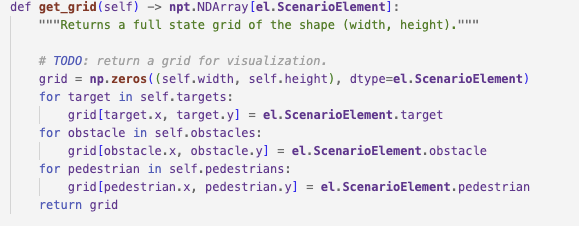
\includegraphics[width=0.5\linewidth]{pictures/Task1 code.png}
      \caption{get grid() method}
      \label{fig:get grid()}
  \end{figure}

\begin{figure}[h]
      \centering
      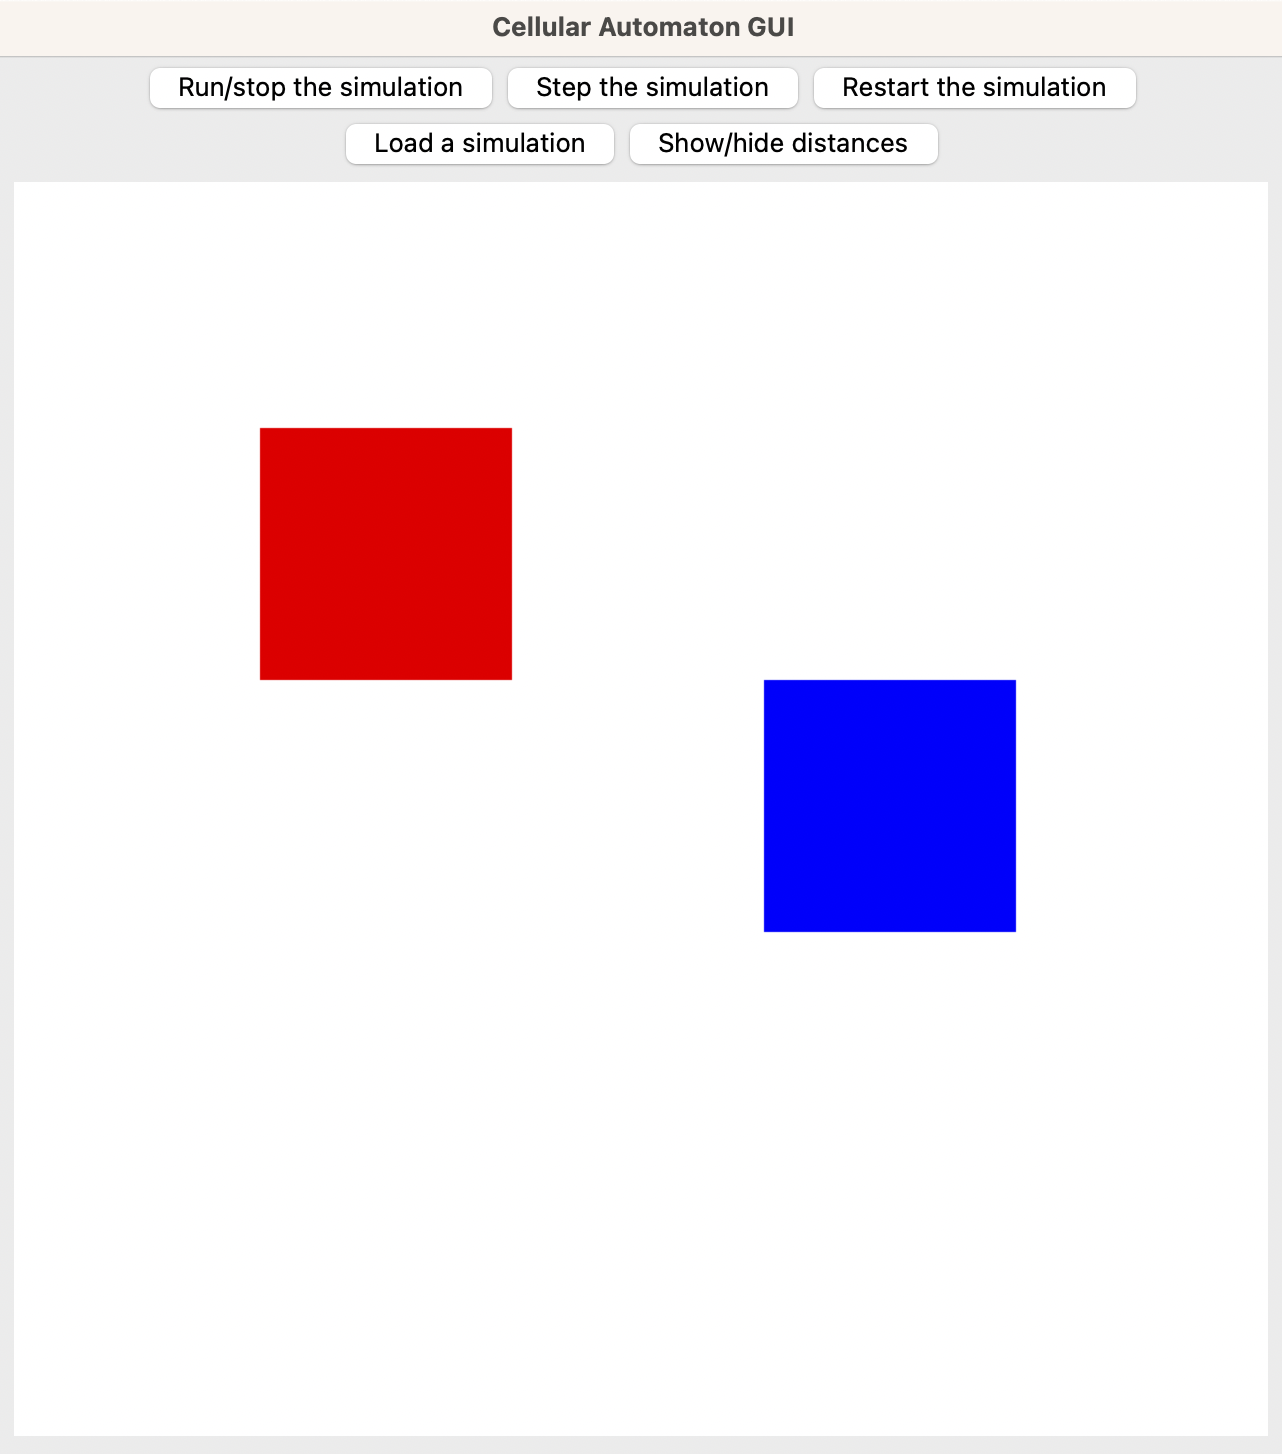
\includegraphics[width=0.5\linewidth]{pictures/Task1.png}
      \caption{The scenario of Task 1}
      \label{fig:The scenario of Task 1}
  \end{figure}
The red ones in the picture represent pedestrians, and the yellow ones represent targets. It can be controlled through the provided GUI. The specific functions are:
\begin{itemize}
    \item Run/Stop the simulation :Clicking on the "Run" button will start the simulation, while clicking on the "Stop" button will pause it.
    \item Step the simulation :Clicking on the "Step" button will execute a single iteration of the simulation.
    \item Restart the simulation :Clicking on the "Restart" button will clear any ongoing simulation progress and return all parameters and entities to their starting positions.
    \item Load a simulation :This function enables users to load a previously saved simulation scenario.
    \item Show/hide distance :This function toggles the display of distance measurements within the simulation environment.
\end{itemize}
The toy example file is a json file that sets a specific scene, which specifies the length and width of the grid, the number and location of pedestrians, target points, obstacles, etc. Using this as an example, other scenarios can be generated for subsequent tasks.
\end{task}

\section{Task 2}

\begin{task}{TASK 2, First step of a single pedestrian}
In this task, it needs to be accomplished to move a single pedestrian to a designated target. First generate the corresponding scene, define a grid with a length and width of 50, set the pedestrian's initial position to (5, 25), and set the target to (25, 25). The pedestrian's speed defaults to 1 unit length per time unit. 
\begin{figure}[h]
      \centering
      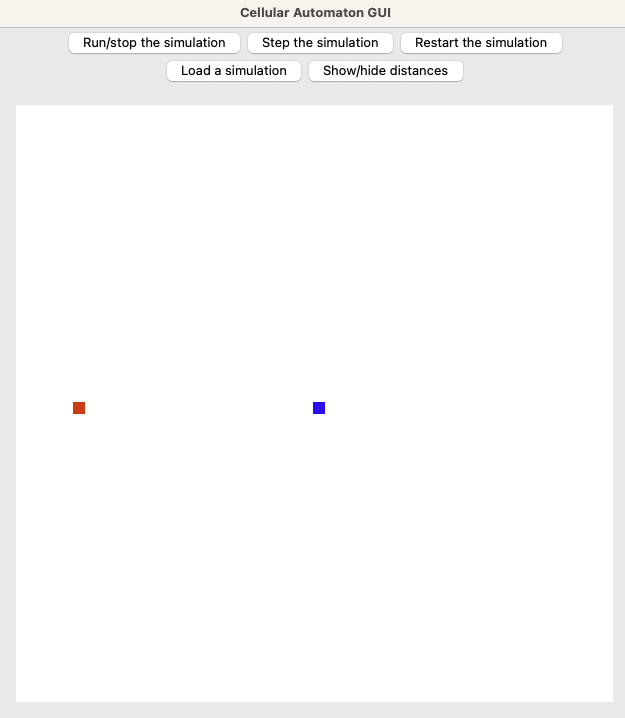
\includegraphics[width=0.35\linewidth]{pictures/Task2_initial .png}
      \caption{Initial state of task 2}
      \label{fig:Initial state of task 2}
  \end{figure}
This is expected to reach the target after 25 time units. Compile the corresponding information into a json file, and obtain the initial situation after visualization. In order to complete this task, the following methods need to be used
\begin{itemize}
    \item \texttt{get\_neighbors()} method :In this method, the coordinates of any point in the grid can be input, and the coordinates of 8 adjacent points will be returned. This is obtained by adding or subtracting 1 to the x and y of the given coordinates respectively.
    \item \texttt{compute\_naive\_distance\_grid} :In this method, the distance between all points in the grid and the nearest target point is calculated, and a matrix with the same shape as the grid is returned.
    \item \texttt{update\_step}:Through the above two methods, the update of each step of the pedestrian can be completed. The specific idea is to obtain the eight neighbors around the pedestrian based on its position, and then calculate the distance between the eight neighbors and the target point through \texttt{compute\_naive\_distance\_grid}. Select the neighbor with the smallest distance and set the next pedestrian's position as the neighbor's position. 
\end{itemize}
After the setting is completed, the pedestrian advances towards the target at a speed of one frame per unit time. After 20 time units, the pedestrian reaches the target.According to the requirements of the question, the pedestrian should be absorbed after reaching the target point, so the method is set to remove the pedestrian when the pedestrian reaches the target point. It can be seen from the visualization results obtained from the GUI that within one time unit after the pedestrian arrives, the color of the target point returns to its original color.

\begin{figure}[h]
  \centering
  \begin{subfigure}[b]{0.4\textwidth}
    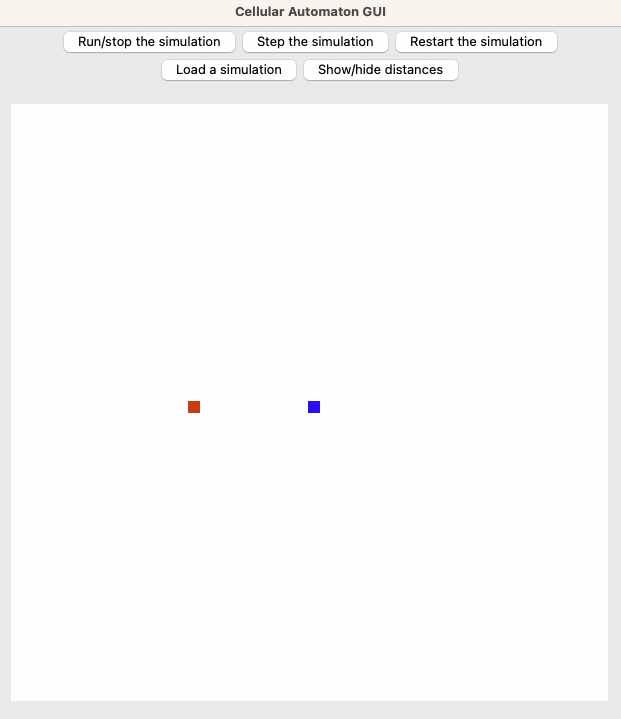
\includegraphics[width=\textwidth]{pictures/Task2_Intermediate state.png}
    \caption{Intermediate state of task 2}
    \label{fig:Intermediate state of task 2}
  \end{subfigure}
  \hfill
  \begin{subfigure}[b]{0.4\textwidth}
    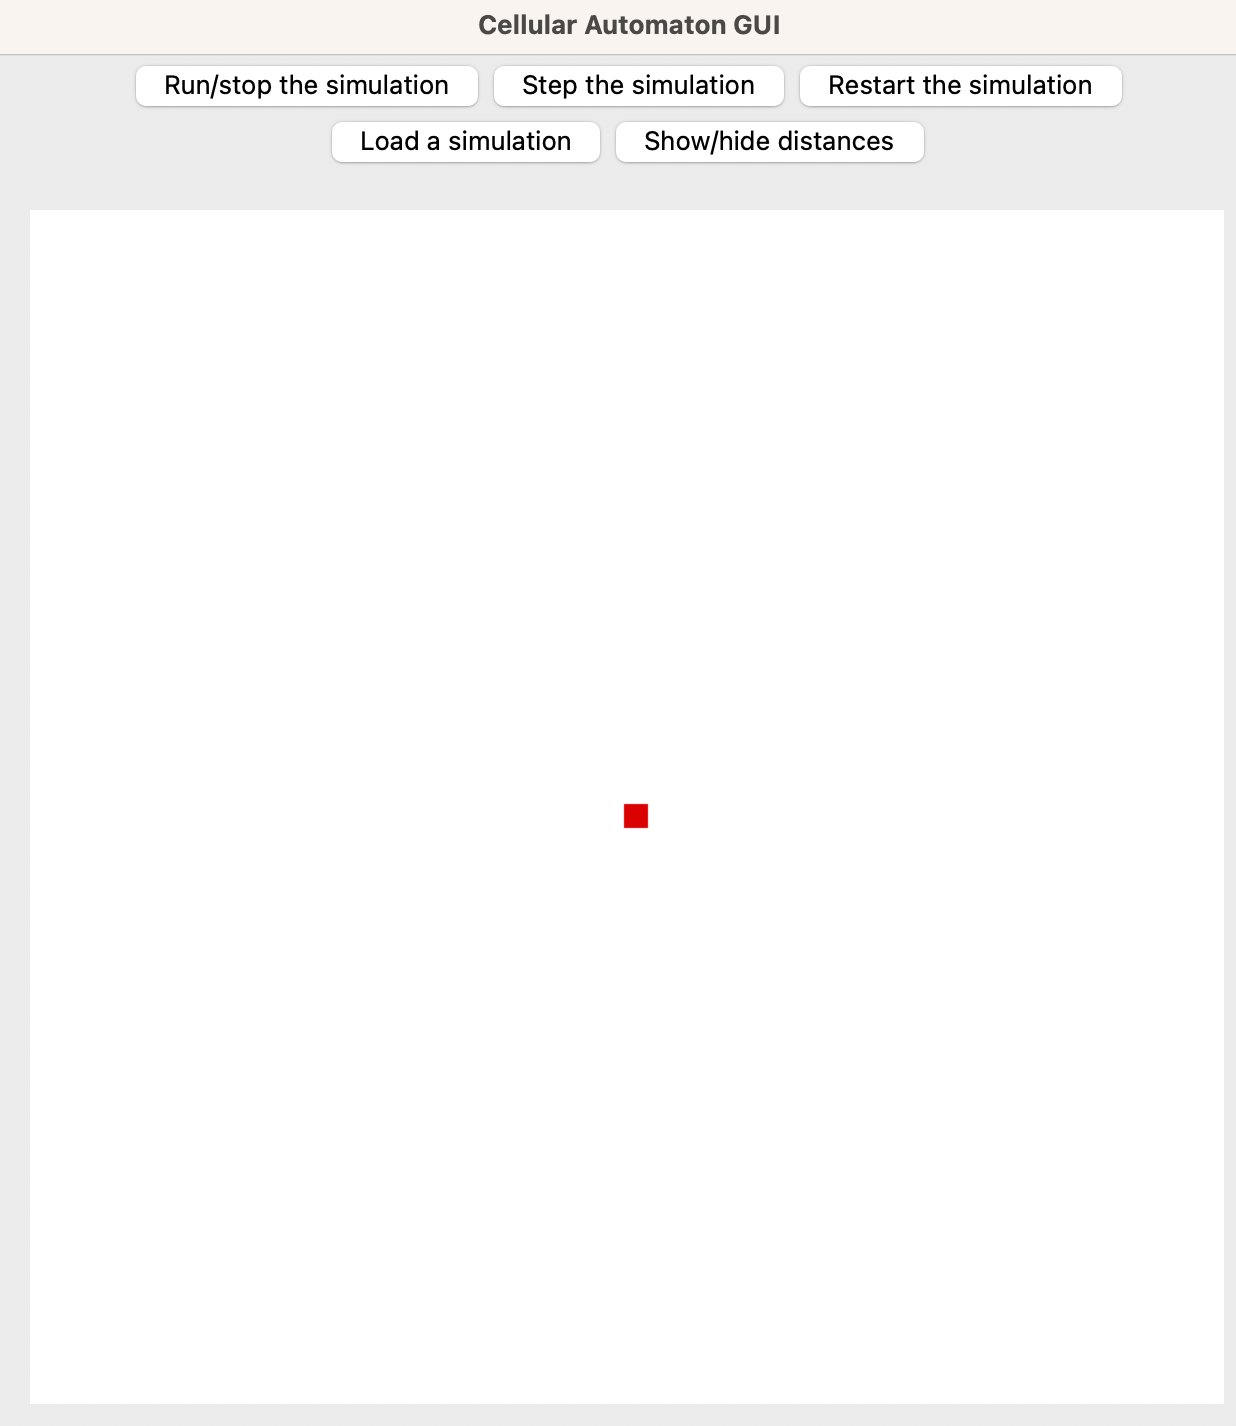
\includegraphics[width=\textwidth]{pictures/Task2_end.png}
    \caption{Final state of task 2}
    \label{fig:Final state of task 2}
  \end{subfigure}
  \caption{Task 2}
  \label{Task 2}
\end{figure}
\end{task}

\section{Task 3}

\begin{task}{TASK 3, Interaction of pedestrians}
In this task it is required to make pedestrians interact with each other and test whether they can move in arbitrary directions. Pedestrians should be absorbed (removed from
the scenario) when arriving at target. The pedestrians are placed on vertices of a regular pentagon with the target on the orthocenter, which means that they are in a equally large distance around the single target and the distance between two neighbored pedestrians is the same for each couple. Besides, it is notable that the word ``distance'' stands for Euclidean distance instead of number of cells.

\subsection{Setup of Scenario}

The file configs/task\_3.json generated by generate\_configs.py saves all the information for this scenario. 

\autoref{fig:Task3_initial} demonstrates the initial scenario of Task 3. The grid size is set as $100 \times 100$, while the target is located at (50, 50), which is assigned as the center of a circle. 5 Pedestrians are placed equally on the circle, whose coordinates are (50, 0), (98, 35), (79, 91), (21, 91), (2, 35), computed by trigonometric functions.


\begin{figure}[htbp]
  \centering
  \begin{subfigure}[b]{0.31\textwidth}
    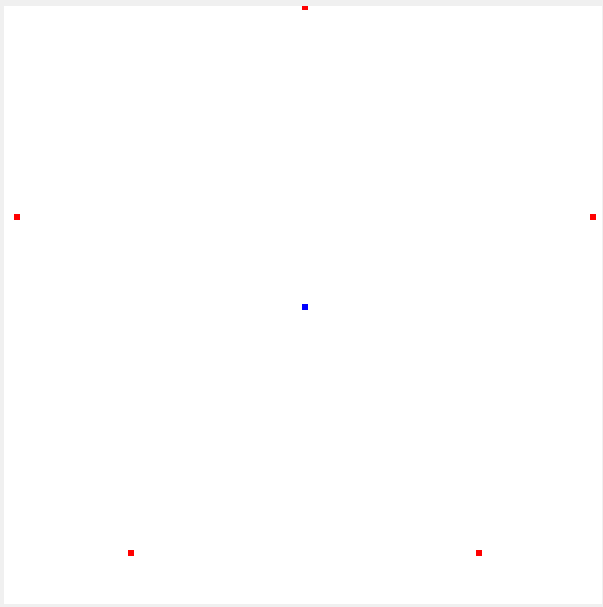
\includegraphics[width=\textwidth]{pictures/Task3_initial.png}
    \caption{Initial state of Task 3}
    \label{fig:Task3_initial}
  \end{subfigure}
  \begin{subfigure}[b]{0.31\textwidth}
    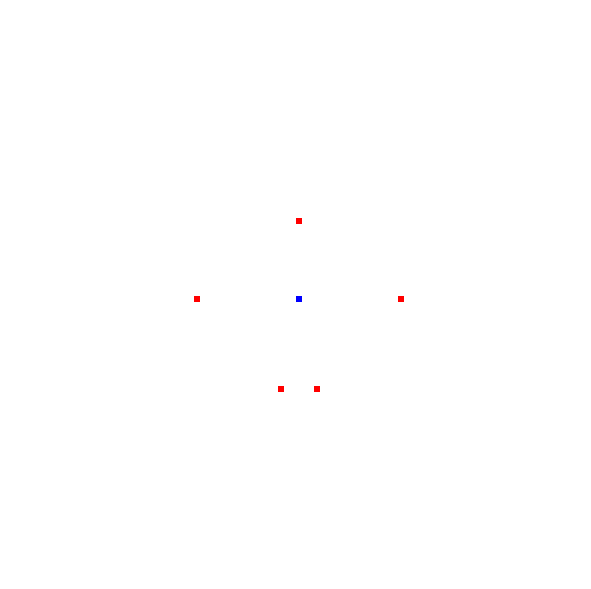
\includegraphics[width=\textwidth]{pictures/Task3_intermediate.png}
    \caption{Intermediate state of Task 3}
    \label{fig:Task3_intermediate}
  \end{subfigure}
  \begin{subfigure}[b]{0.31\textwidth}
    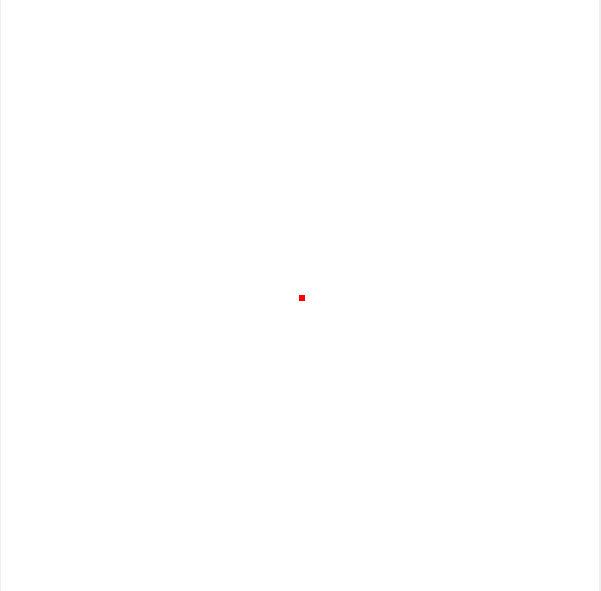
\includegraphics[width=\textwidth]{pictures/Task3_end.png}
    \caption{Final state of Task 3}
    \label{fig:Task3_end}
  \end{subfigure}
  \caption{Visualization of Task 3}
  \label{fig:task3}
\end{figure}


\subsection{Pedestrian Avoidance}

Bresenham’s algorithm is widely used to draw line primitives (straight lines) in bitmap images. Shown in \autoref{fig:Bresenham}, it works with integer coordinates and uses only integer addition, subtraction, and bit shifting operations, making the computation efficient\cite{bolder2001high}. In the implementation of pedestrian or obstacle detection, each pedestrian is supposed to move from one to next possible position along Bresenham path. If the Bresenham path is blocked by other objects, this possible position will be abandoned.

\begin{figure}
    \centering
    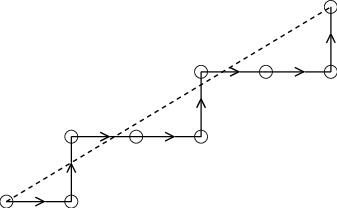
\includegraphics[width=0.5\linewidth]{pictures/Bresenham.png}
    \caption{Bresenham path}
    \label{fig:Bresenham}
\end{figure}

The function avoidance\_cost is used to implement pedestrian avoidance, which is adapted from the cost function in exercise sheet. For one pedestrian in an update step, the function takes other pedestrians into consideration, who are in the Bresenham path of that pedestrian to the next position. Afterwards it computes the avoidance costs (\autoref{eq:avoidance_cost}) between that pedestrian and each filtered pedestrian and sums them up. The endure\_factor k is introduced to adjust the maximum of the cost. Smaller k reflects weaker avoidance among the pedestrians, which indicates that they tend to endure the crowd to a greater extent. The value 0.01 is to avoid extreme cases where $r = r_max$ and the denominator thus becomes 0, which makes the cost go to infinity.

\begin{align}
    \label{eq:avoidance_cost}
    c(r)=\left\{\begin{array}{cc}
    k \cdot \exp \left(\frac{1}{r^{2}-r_{\max }^{2} + 0.01}\right) & \text { if } r<r_{\max } \\
    0 & \text { else }
    \end{array}\right.
\end{align}

\subsection{Speed Adjustment}

The speed adjustment is designed as follows. When the above-mentioned avoidance cost of a pedestrian is equal to 0, which means there is no other pedestrian in the forward direction, the pedestrian will increase the speed by 3\%. In order to prevent them from moving too fast, the speed will not increase after it exceeds 1.2 times the initial speed. When the avoidance cost is not equal to 0, the pedestrian will maintain the initial speed. When the distance of the pedestrian to the targets is small enough that he/she can arrive at the targets at next time step, the speed will decrease to avoid overshooting by the function near\_target\_adjustment().

\subsection{Simulation}

The speed of each pedestrian is set to 5. When running the scenario, all the pedestrians move in a direction to the target at the center and reach the target one after another, approximately at the same time. The traveling time is 10s, 12s, 13s, 14s and 15s, respectively, which corresponds to the estimated speed $v = 50 / (5s^{-1}) = 10s$.

\end{task}

\section{Task 4}

\begin{task}{TASK 4, Obstacle avoidance}

\subsection{Setup of Scenarios}
There are 2 scenarios in Task 4, ``bottleneck'' and ``chicken test''. 

In ``bottleneck'' scenario, the narrow corridor ($5m \times 1m $) connects 2 large squared rooms ($10m \times 10m$). The two ends of the corridor are located at the middle points of the two walls. 150 people, located in the left half of the room on the left, are heading towards the exit in the middle of the wall on the right side of the right room.

In ``chicken test'', 150 people are supposed to bypass a U-shaped room with 3 walls. They are facing the entrance of the room, while the target is located to the right of the room. Inappropriate implementation of obstacle avoidance may cause the crowd to get stuck in the room.


\subsection{Rudimentary Obstacle Avoidance}
%Rudimentary obstacle avoidance is realized by a function named find\_best\_neighbor(). , it will search the neighbors of that position.
If one of the neighbors is a target, it will be the next possible position. In most instances, none of the neighbors is a target and the pedestrian will get the next possible position by its current speed and the direction to each neighbor. The direction is achieved by calculating cosine and sine of the angle between the pedestrian and each neighbor.

A set called ``blocks'' include the real-time coordinates of every obstacle and pedestrian except the specified one. When the coordinates of cells on Bresenham path from current position to next possible position are in the set ``blocks'', the neighbor corresponding to this possible position will be set to have an infinite avoidance cost, which makes the pedestrian avoid this direction later.

To avoid stepping back, the computed distance of a pedestrian to the target is required to get smaller or at least stay unchanged.

After that, it will find the neighbor with the smallest avoidance cost and obtain the direction at next step.

Therefore, the rudimentary obstacle avoidance will be carried out simultaneously with the pedestrian avoidance. The difference is that no avoidance cost between pedestrians and obstacles is calculated and included in total costs.
%select the nearest neighbor of that position to himself/herself as the newer potential position

\subsection{Dijkstra Algorithm}

In crowd modeling and simulation, Dijkstra algorithm is often used to find the shortest path from one point to another within a simulated environment. A function named \_compute\_dijkstra\_distance\_grid(self, targets: tuple[utils.Position]) -\textgreater npt.NDArray[np.float64] is defined to implement Dijkstra algorithm. This function initializes a distance grid filled with infinity values and set the values at targets to be 0. It adds each target to the ``edge'' list with a priority of 0, which includes their coordinates. The main loop continues until there are no more nodes in edge. In the loop, it extracts the node with the smallest distance (min\_node\_value) and its coordinates (min\_node) from edge. The neighboring cells' coordinates (new\_x, new\_y) in 8 directions are obtained and it will check if the new position is within the grid bounds and not an obstacle. The movement cost is to be calculated: 1.414213562373095 for diagonal moves (since diagonals in a grid have a length of $\sqrt{2}$) and 1 for straight moves. If moving to (new\_x, new\_y) offers a shorter path than previously known (distances[new\_x, new\_y] \textgreater min\_node\_value + cost), update the distance and push the new position with its updated distance into ``edge'' list. Once the priority queue ``edge'' list is empty, indicating all reachable cells have been evaluated, the function returns the array of distance grid, which contains the shortest distances from any of the target positions to all other positions, considering obstacles. \autoref{fig:distance_visualization} gives a visualization of Dijkstra distances, where the darker the color, the greater is the distance value.

\begin{figure}
    \centering
    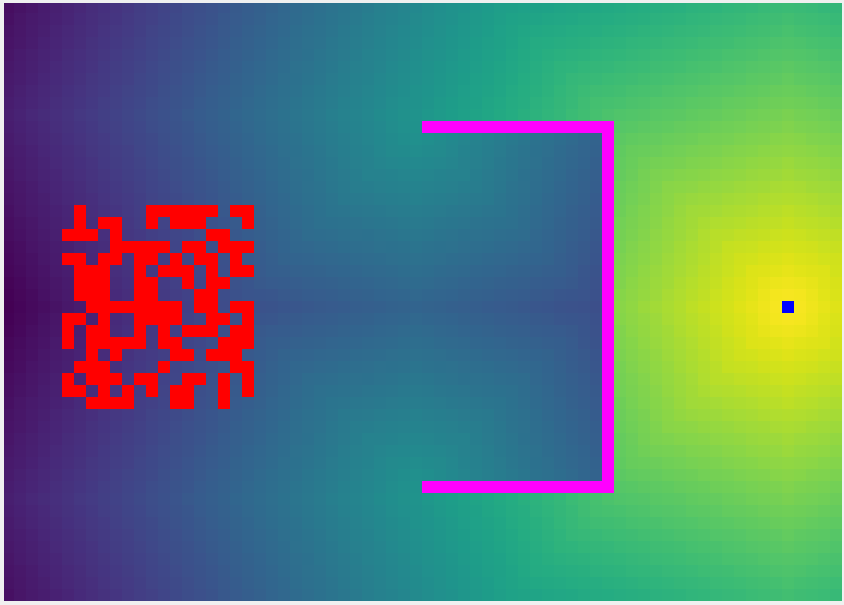
\includegraphics[width=0.5\linewidth]{distance_visualization.png}
    \caption{The visualization of Dijkstra distances in ``chicken test''}
    \label{fig:distance_visualization}
\end{figure}

\subsection{Results of Simulation}

\autoref{fig:task4cr} and \autoref{fig:task4cd} compare the simulation of ``chicken test'' with rudimentary obstacle avoidance to that with Dijkstra algorithm. In the simulation with rudimentary obstacle avoidance, the crowd fails to detect the whole form of the U-shaped obstacle and gets totally stuck in the end, without any pedestrian getting out of the trap. In contrast, with Dijkstra algorithm, the crowd is separated into two groups, going upwards and downwards. The pedestrians manage to bypass the obstacles and arrive at the target one by one. Therefore, Dijkstra algorithm is more effective in ``chicken test"" scenario.



\begin{figure}[htbp]
  \centering
  \begin{subfigure}[b]{0.31\textwidth}
    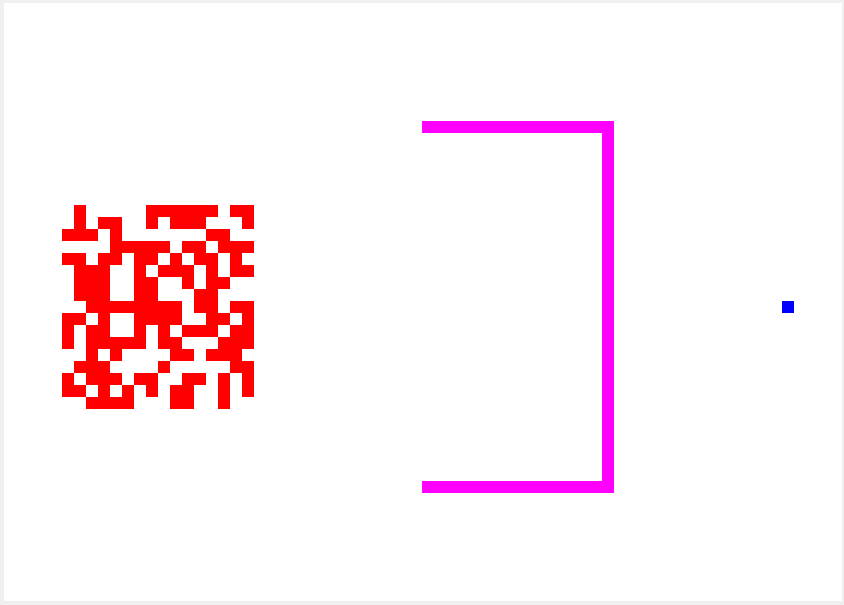
\includegraphics[width=\textwidth]{pictures/Task4_initial_cr.png}
    \caption{Initial state}
    \label{fig:Task4_initial_cr}
  \end{subfigure}
  \begin{subfigure}[b]{0.31\textwidth}
    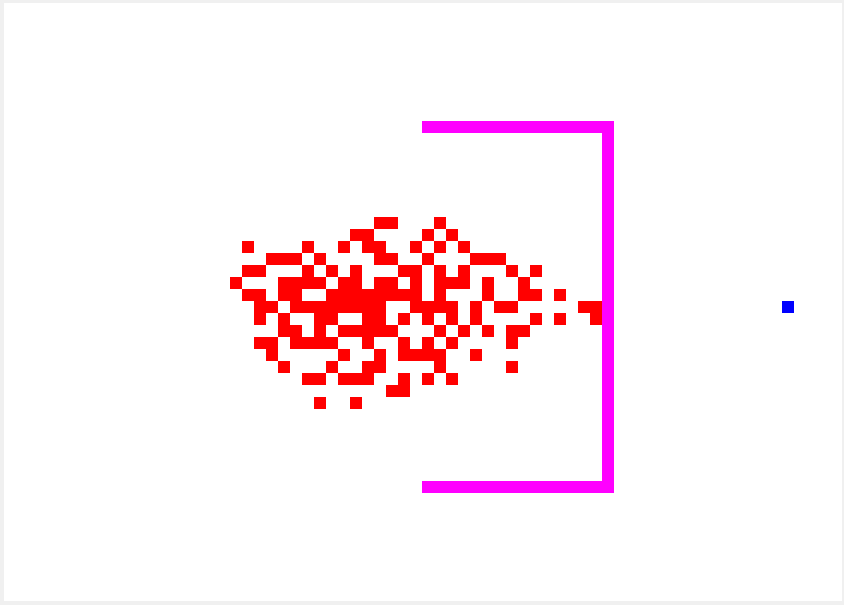
\includegraphics[width=\textwidth]{pictures/Task4_intermediate_cr.png}
    \caption{Intermediate state}
    \label{fig:Task4_intermediate_cr}
  \end{subfigure}
  \begin{subfigure}[b]{0.31\textwidth}
    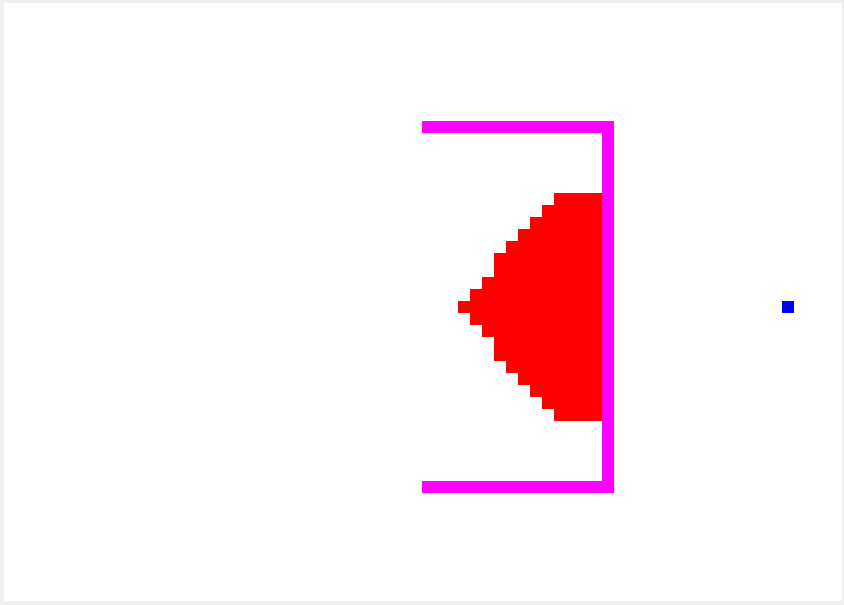
\includegraphics[width=\textwidth]{pictures/Task4_end_cr.png}
    \caption{State near the end}
    \label{fig:Task4_end_cr}
  \end{subfigure}
  \caption{Visualization of ``chicken test'' in Task 4, with rudimentary obstacle avoidance}
  \label{fig:task4cr}
\end{figure}

\begin{figure}[htbp]
  \centering
  \begin{subfigure}[b]{0.31\textwidth}
    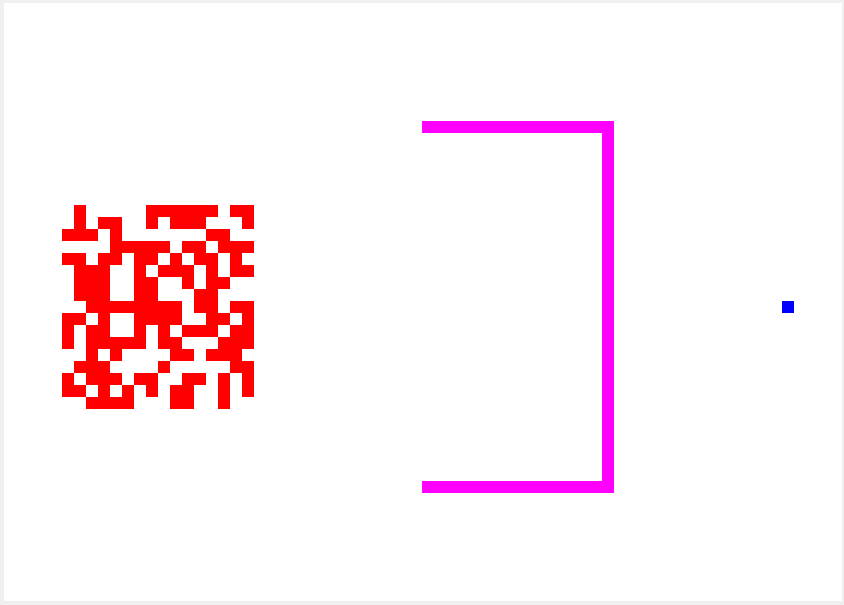
\includegraphics[width=\textwidth]{pictures/Task4_initial_cd.png}
    \caption{Initial state}
    \label{fig:Task4_initial_cd}
  \end{subfigure}
  \begin{subfigure}[b]{0.31\textwidth}
    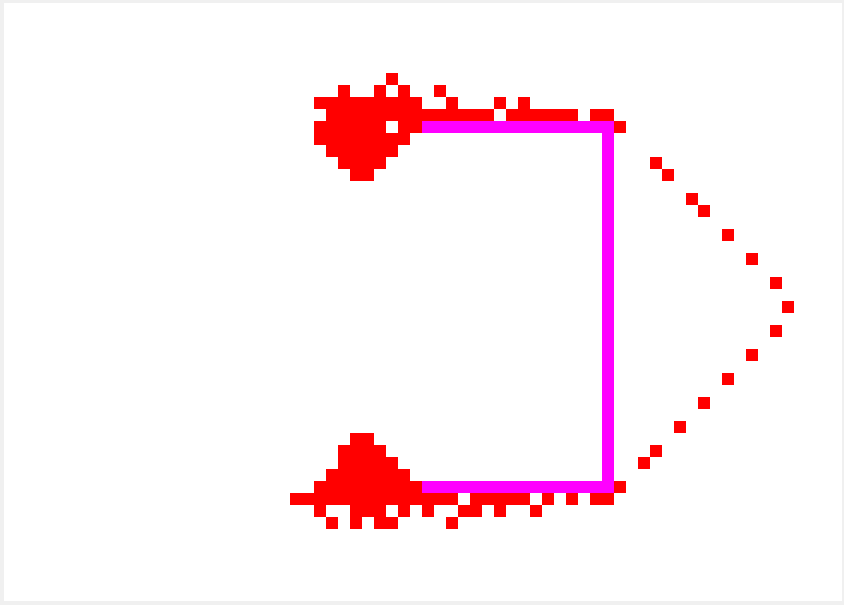
\includegraphics[width=\textwidth]{pictures/Task4_intermediate_cd.png}
    \caption{Intermediate state}
    \label{fig:Task4_intermediate_cd}
  \end{subfigure}
  \begin{subfigure}[b]{0.31\textwidth}
    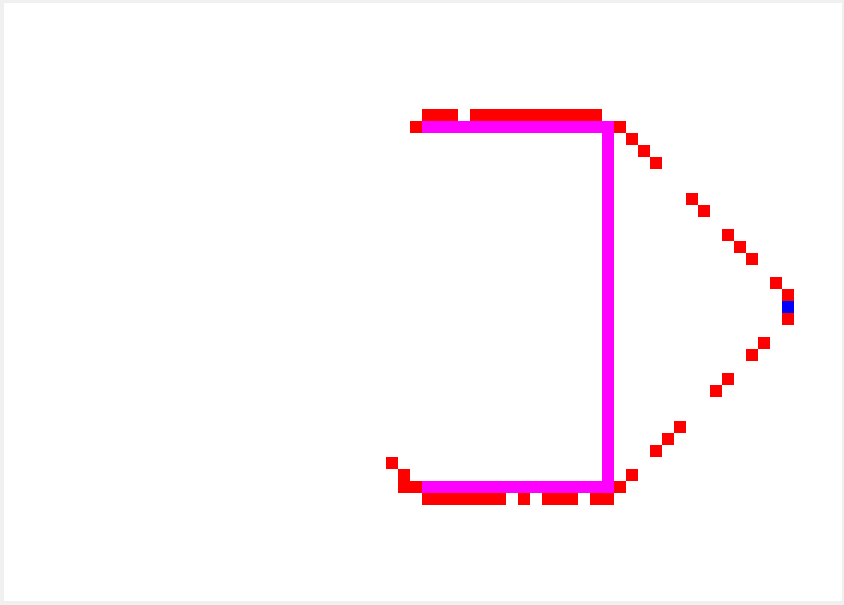
\includegraphics[width=\textwidth]{pictures/Task4_end_cd.png}
    \caption{State near the end}
    \label{fig:Task4_end_cd}
  \end{subfigure}
  \caption{Visualization of ``chicken test'' in Task 4, with Dijkstra algorithm}
  \label{fig:task4cd}
\end{figure}

\autoref{fig:task4br} and \autoref{fig:task4bd} compare the simulation of ``bottleneck'' with rudimentary obstacle avoidance to that with Dijkstra algorithm. In the simulation with rudimentary obstacle avoidance, the crowd gather heavily on both sides of the bottleneck entrance. However, they can still reach the target after a relatively long time. In contrast, with Dijkstra algorithm, the crowd seems to stand in a line before going through the bottleneck. There is no gathering on both sides, which makes the crowd move smoothly. In the end, all of the pedestrians get to the target more quickly. As a comparison, the evacuation time of the former scenario ranges from 51s to 168s, while that of the latter scenario ranges from 51s to 142s, which indicates that Dijkstra algorithm is more efficient in ``bottleneck'' scenario.

\begin{figure}[htbp]
  \centering
  \begin{subfigure}[b]{0.31\textwidth}
    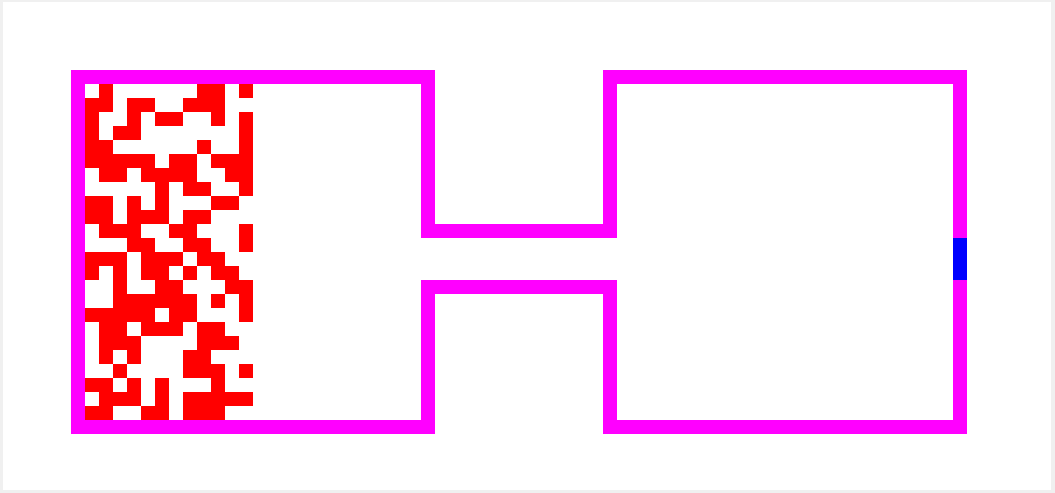
\includegraphics[width=\textwidth]{pictures/Task4_initial_br.png}
    \caption{Initial state}
    \label{fig:Task4_initial_br}
  \end{subfigure}
  \begin{subfigure}[b]{0.31\textwidth}
    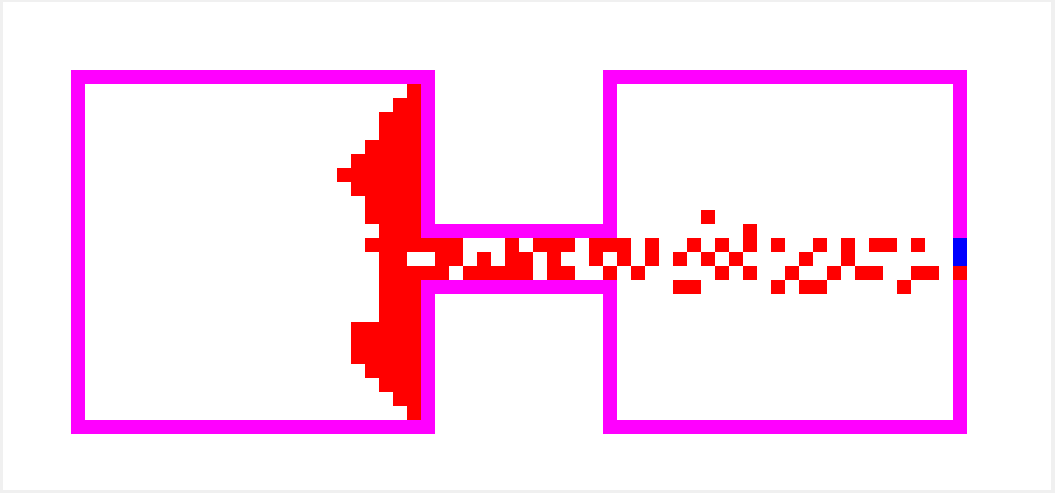
\includegraphics[width=\textwidth]{pictures/Task4_intermediate_br.png}
    \caption{Intermediate state}
    \label{fig:Task4_intermediate_br}
  \end{subfigure}
  \begin{subfigure}[b]{0.31\textwidth}
    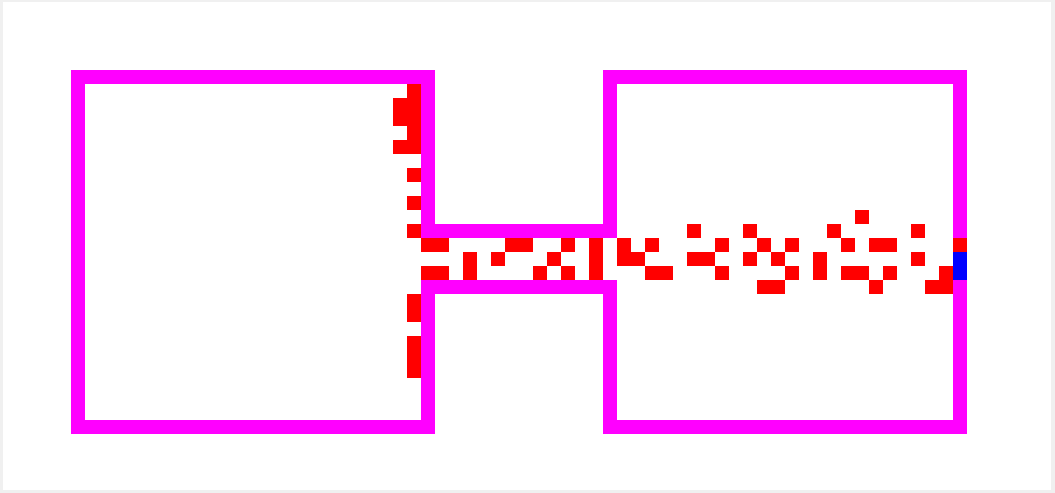
\includegraphics[width=\textwidth]{pictures/Task4_end_br.png}
    \caption{State near the end}
    \label{fig:Task4_end_br}
  \end{subfigure}
  \caption{Visualization of ``bottleneck'' in Task 4, with rudimentary obstacle avoidance}
  \label{fig:task4br}
\end{figure}

\begin{figure}[htbp]
  \centering
  \begin{subfigure}[b]{0.31\textwidth}
    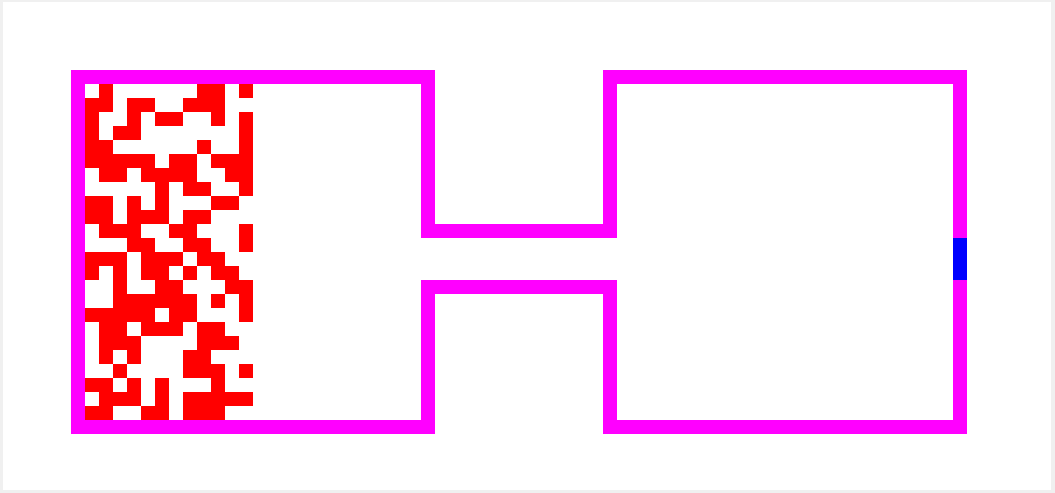
\includegraphics[width=\textwidth]{pictures/Task4_initial_bd.png}
    \caption{Initial state}
    \label{fig:Task4_initial_bd}
  \end{subfigure}
  \begin{subfigure}[b]{0.31\textwidth}
    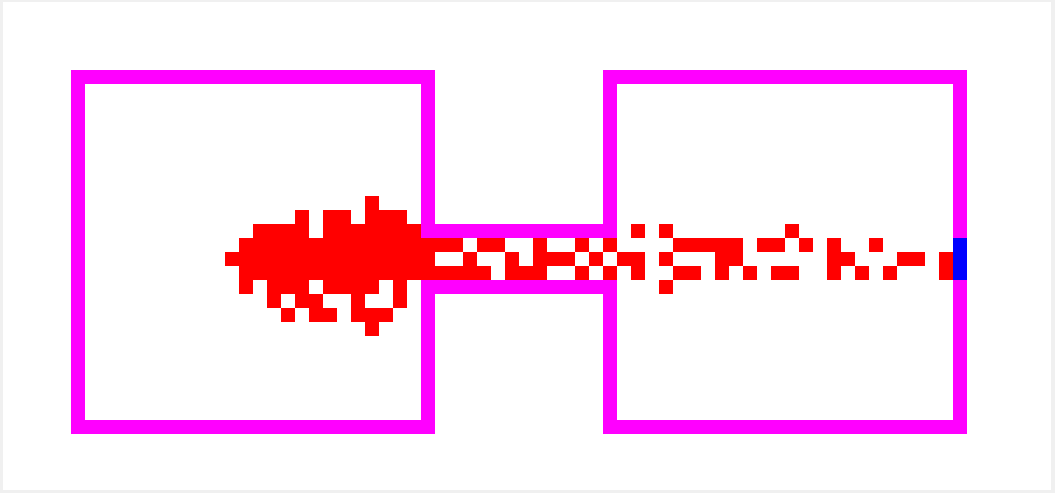
\includegraphics[width=\textwidth]{pictures/Task4_intermediate_bd.png}
    \caption{Intermediate state}
    \label{fig:Task4_intermediate_bd}
  \end{subfigure}
  \begin{subfigure}[b]{0.31\textwidth}
    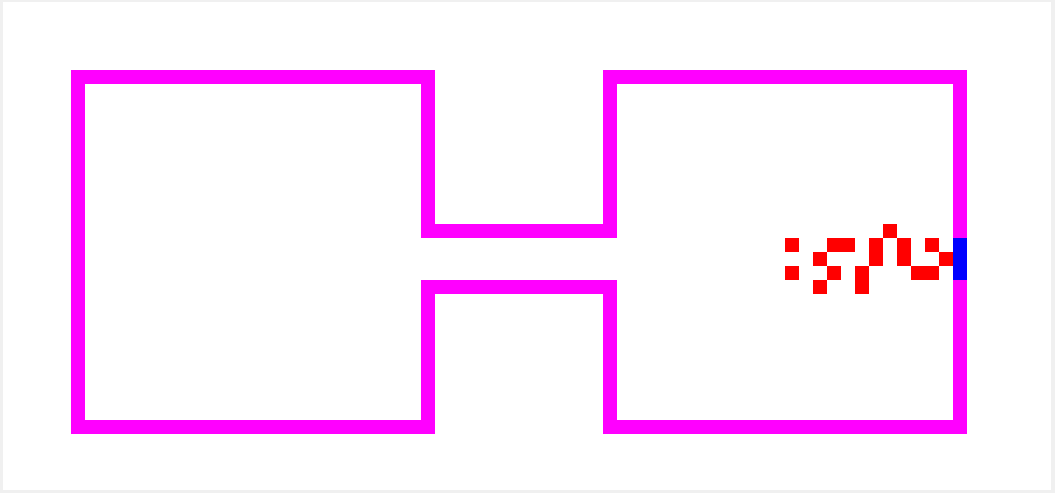
\includegraphics[width=\textwidth]{pictures/Task4_end_bd.png}
    \caption{State near the end}
    \label{fig:Task4_end_bd}
  \end{subfigure}
  \caption{Visualization of ``bottleneck'' in Task 4, with Dijkstra algorithm}
  \label{fig:task4bd}
\end{figure}

\end{task}

\section{Task 5}

\begin{task}{TASK 5, RiMEA tests}

\subsection{Test 1: RiMEA Scenario 1, Maintaining the specified walking speed in a corridor}

\subsubsection{Setup of Scenario}

The scenario is a 40m long and 2 m wide corridor and a pedestrian placed on one end of the corridor is supposed to move in a straight line with correct speed towards the target on the other end. No obstacle is set along the path. Each cell is $0.4m \times 0.4m$, so the corridor excluding borders occupies the zone of $100 \times 5$ cells. The initial speed of the pedestrian is $1.33m/s = (1.33m/s) / (0.4m/cells) \approx 3.33 \enspace cells/s$. The estimated travel time is $40m / 1.33m/s \approx 30.08s $ and the RiMEA requires it to range from 26 to 34 seconds.

\subsubsection{Results of Simulation}

\autoref{fig:test1} illustrates the simulation of Test 1. The pedestrian moves in a straight line and the travel time output in the terminal tells the travel time is $30s$, which is within the given range. After multiple tests, the results remain unchanged, verifying the stability of the algorithm.

\begin{figure}[htbp]
  \centering
  \begin{subfigure}[b]{0.31\textwidth}
    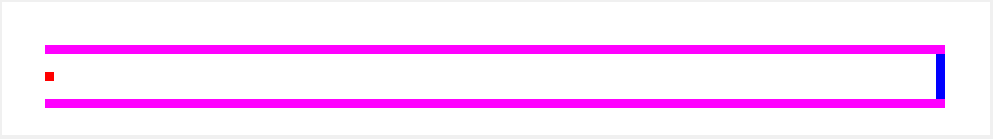
\includegraphics[width=\textwidth]{pictures/test1_initial.png}
    \caption{Initial state}
    \label{fig:test1_initial}
  \end{subfigure}
  \begin{subfigure}[b]{0.31\textwidth}
    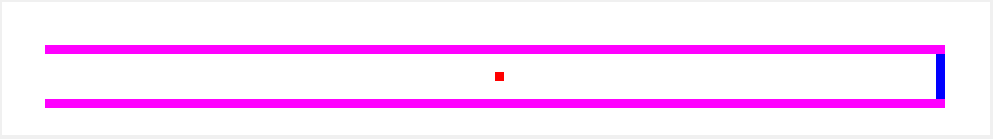
\includegraphics[width=\textwidth]{pictures/test1_intermediate.png}
    \caption{Intermediate state}
    \label{fig:test1_intermediate}
  \end{subfigure}
  \begin{subfigure}[b]{0.31\textwidth}
    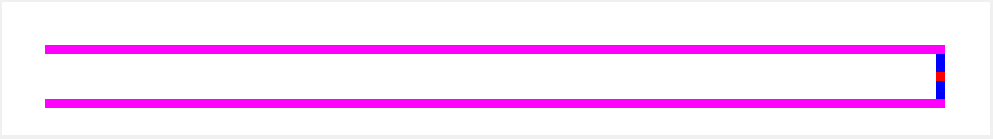
\includegraphics[width=\textwidth]{pictures/test1_end.png}
    \caption{Final state}
    \label{fig:test1_end}
  \end{subfigure}
  \caption{Visualization of Test 1 in Task 5}
  \label{fig:test1}
\end{figure}


\subsection{Test 2: RiMEA Scenario 4}

\subsubsection{Setup of Scenario}

\autoref{fig:test2_setup} depicts the setup of Test 2\cite{RimeaGuidelines2016}, which is a $1000m$ (2500 cells) long and $10m$ (25 cells) wide corridor), where there are three measuring points ($2m \times 2m$ or $5 \times 5$ cells). However, this scenario requires huge computational resources. In order to complete the test, the scenario size should be reduced. The cell size is $0.4m \times 0.4m$. The cut-down corridor $16m$ (40 cells) long and $7.6m$ (19 cells) wide. The corridor is to be filled with different densities of persons with free walking speed ($1.2 - 1.4m/s$): $0.5 P/m^{2}, 1 P/m^{2}, 2 P/m^{2}, 3 P/m^{2}, 4 P/m^{2}, 5 P/m^{2}, 6 P/m^{2}$. Each of the measuring point contains $3 \times 3$ cells. The coordinates of top-left cells of the measuring points are $(29, 10), (35, 10), (35, 13)$.

To get the number of pedestrians in the displayed zone, densities will be multiplied by the area of this zone ($16m \times 7.6m = 121.6m^{2}$). The average speed of individuals is to be calculated at designated measurement points across a 6-second interval, given a specified density. The initial 2 seconds of data may be disregarded as they represent a "transient response". Based on the collected data average speed in the range of a measuring point, the flow of the individuals at a measuring point can be calculated by $flow = speed \times n$, where $n$ is the number of people per square meter in a measuring point. After the measuring time is over, the average of the flows over every time step during measuring time will be calculated and output in the terminal, which is recorded and plotted.

\begin{figure}[htbp]
      \centering
      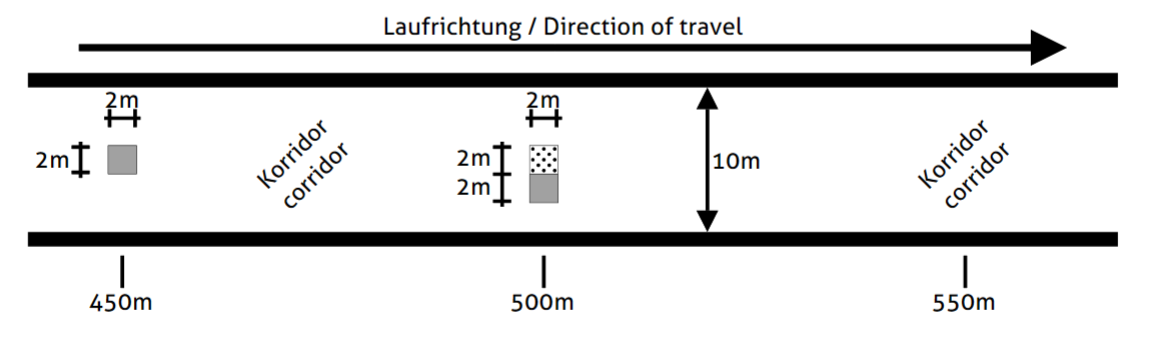
\includegraphics[width=0.9\linewidth]{pictures/test2_setup.png}
      \caption{The setup of Test 2 in Task 5}
      \label{fig:test2_setup}
\end{figure}

\subsubsection{Results of Simulation}

As shown in \autoref{fig:test2}, 7 scenarios with $density = 0.5, 1, 2, ... 6 P/m^2$ are modeled. \autoref{fig:measured_flow_density} demonstrates the relationship between flow and density. At measuring point 1, 2 and 3, the flow reaches its maximum when density is equal to 2, 3 and 2, respectively. As density increases, flow increases to maximum and then decreases, which is reasonable, because the space of the scenario is limited and the flow must have an upper limit. When the preassigned density is small enough, the pedestrians can maintain initial speeds and the flow increases with density. When the preassigned density gets larger, the pedestrians slow down and the flow reduces with density.

The exercise sheet raises questions for this test: why can the premovement time be ignored for the tests? Why is the body size (e.g., the cell size in meters) needed to complete the tests? 

During the premovement time the measurement is deactivated, making the crowd get ready to start walking. There are always pedestrians of the same distribution getting through the measuring points regardless of the premovement time so that it doesn't affect the measurement. In comparison, cell size contributes to the calculation of the flow. $\text{flow} = \frac{\text{average speed (cells/s)} \times \text{cell size (m/cell)} \times n (\text{Persons}) }{\text{width (cells)} \times \text{cell size (m/cell)} \times \text{height (cells)} \times \text{cell size (m/cell)}} = \frac{\text{average speed (cells/s)} \times n (\text{Persons})}{\text{width (cells)} \times \text{cell size (m/cell)} \times \text{height (cells)}}$, including the variable cell size. Therefore, measured flow is inversely proportional to cell size, which can't be neglected.
%flow = average speed (cells/s) * n (Persons) / width (cells) / height (cells) = average speed (cells/s) * cell size (m/cell) * n (Persons) / (width (cells) * cell size (m/cell))  / (height (cells) * cell size (m/cell)) = average speed (cells/s) * n (Persons) / (width (cells) * cell size (m/cell))  / (height (cells)) 


\begin{figure}[htbp]
  \centering
  \begin{subfigure}[b]{0.31\textwidth}
    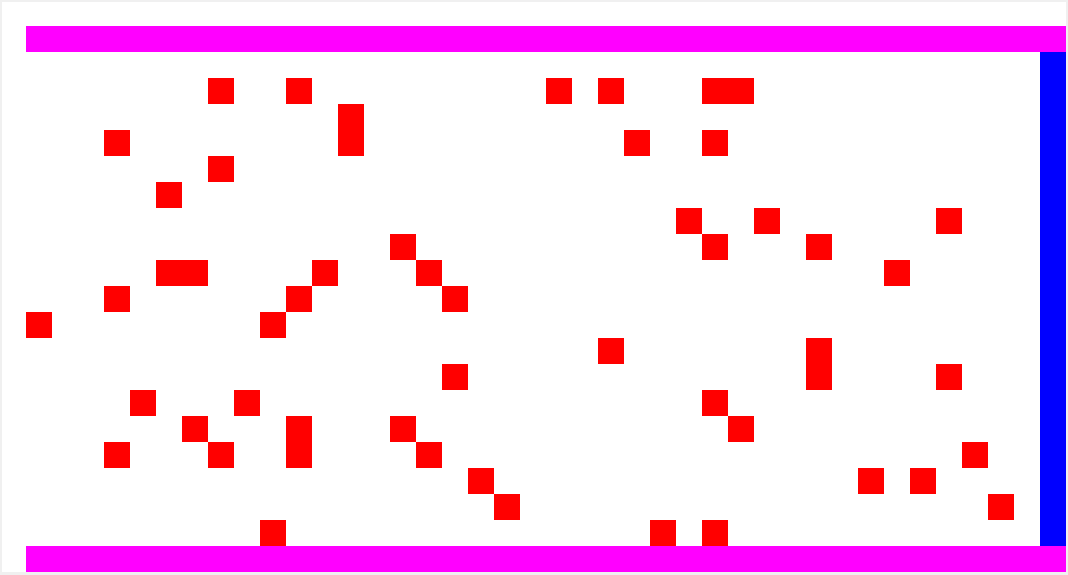
\includegraphics[width=\textwidth]{pictures/test2_0.5.png}
    \caption{$Density = 0.5 P/m^2$}
    \label{fig:test2_0.5}
  \end{subfigure}
  \begin{subfigure}[b]{0.31\textwidth}
    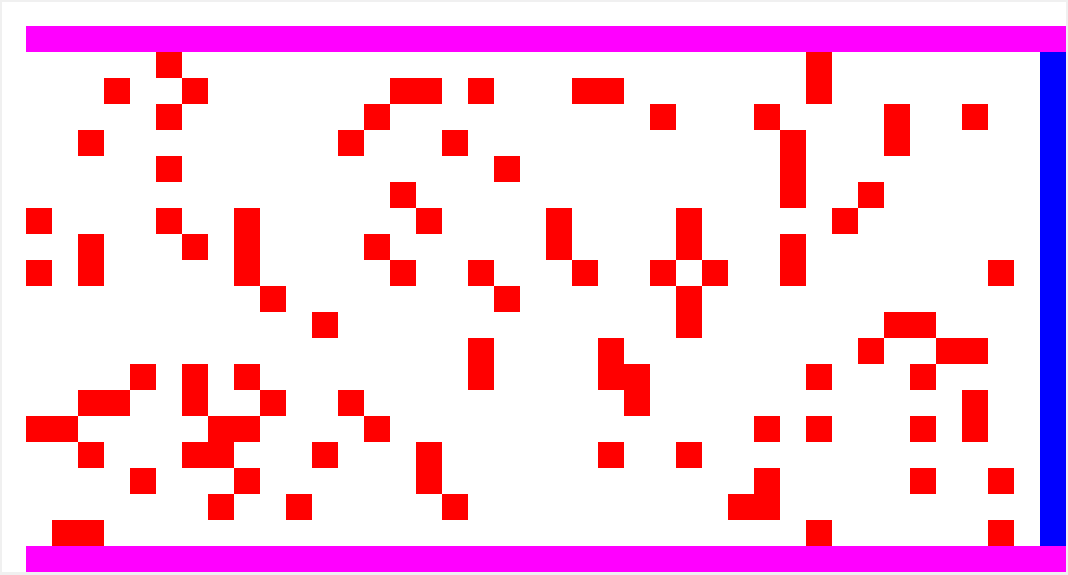
\includegraphics[width=\textwidth]{pictures/test2_1.png}
    \caption{$Density = 1 P/m^2$}
    \label{fig:test2_1}
  \end{subfigure}
  \begin{subfigure}[b]{0.31\textwidth}
    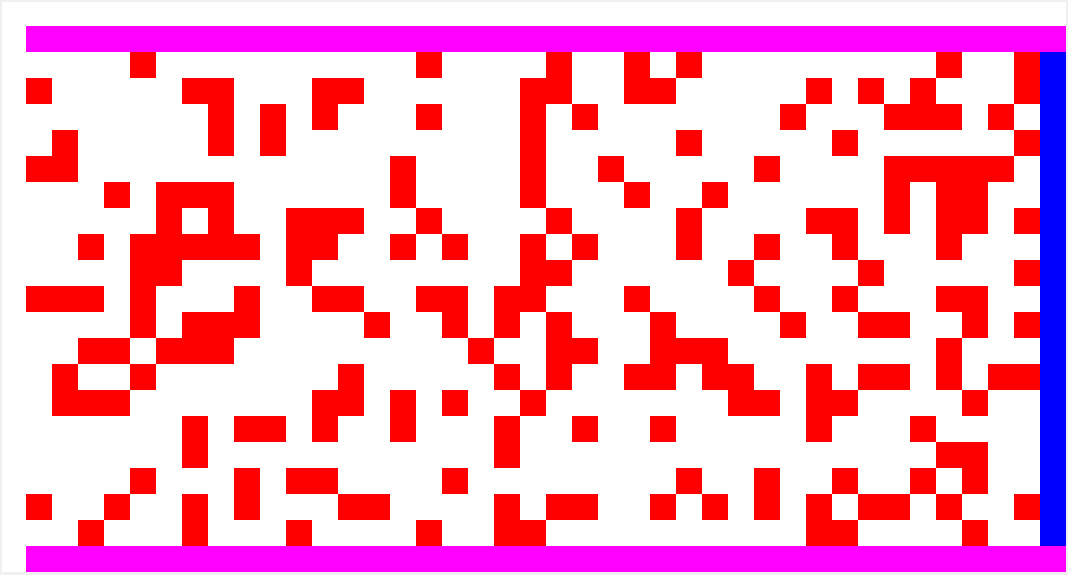
\includegraphics[width=\textwidth]{pictures/test2_2.png}
    \caption{$Density = 2 P/m^2$}
    \label{fig:test2_2}
  \end{subfigure}
  \begin{subfigure}[b]{0.31\textwidth}
    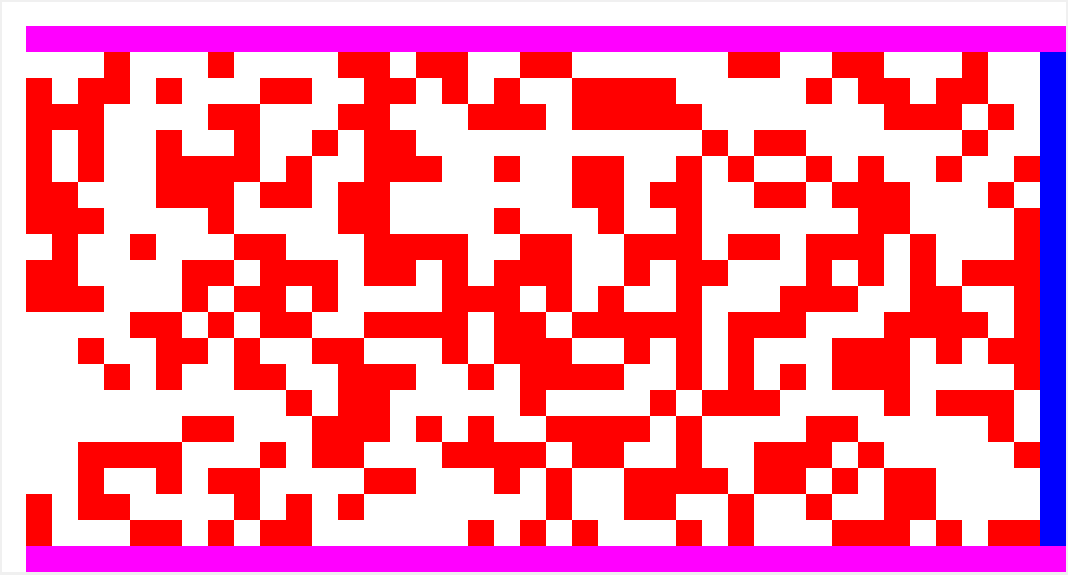
\includegraphics[width=\textwidth]{pictures/test2_3.png}
    \caption{$Density = 3 P/m^2$}
    \label{fig:test2_3}
  \end{subfigure}
  \begin{subfigure}[b]{0.31\textwidth}
    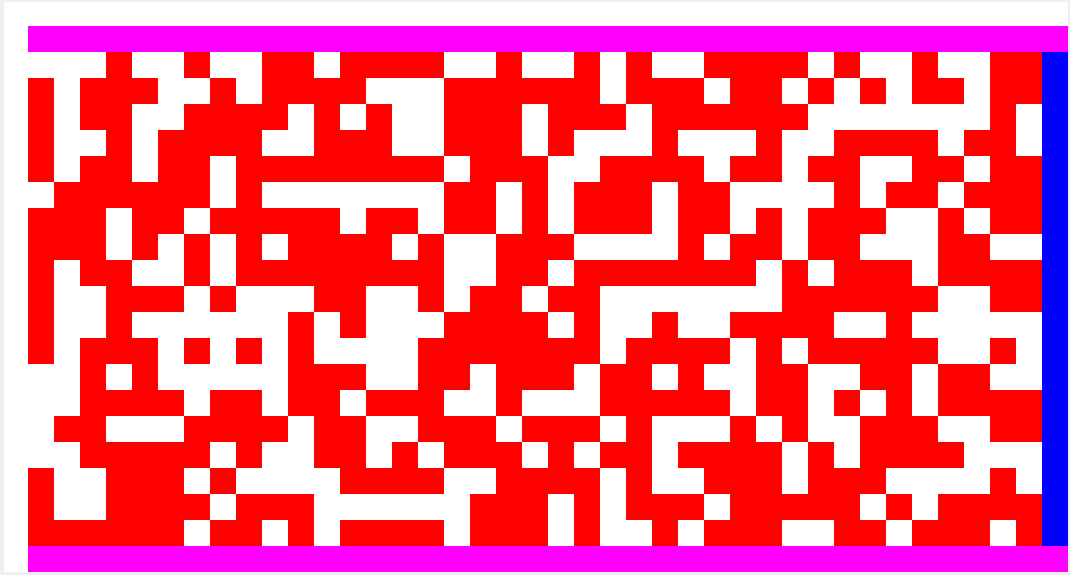
\includegraphics[width=\textwidth]{pictures/test2_4.png}
    \caption{$Density = 4 P/m^2$}
    \label{fig:test2_4}
  \end{subfigure}
  \begin{subfigure}[b]{0.31\textwidth}
    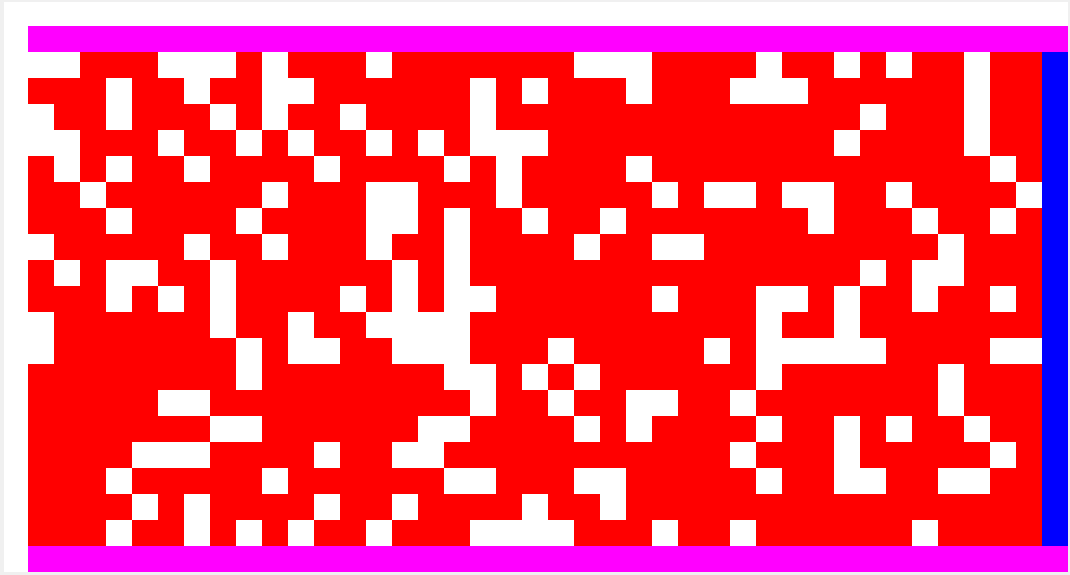
\includegraphics[width=\textwidth]{pictures/test2_5.png}
    \caption{$Density = 5 P/m^2$}
    \label{fig:test2_5}
  \end{subfigure}  
  \begin{subfigure}[b]{0.31\textwidth}
    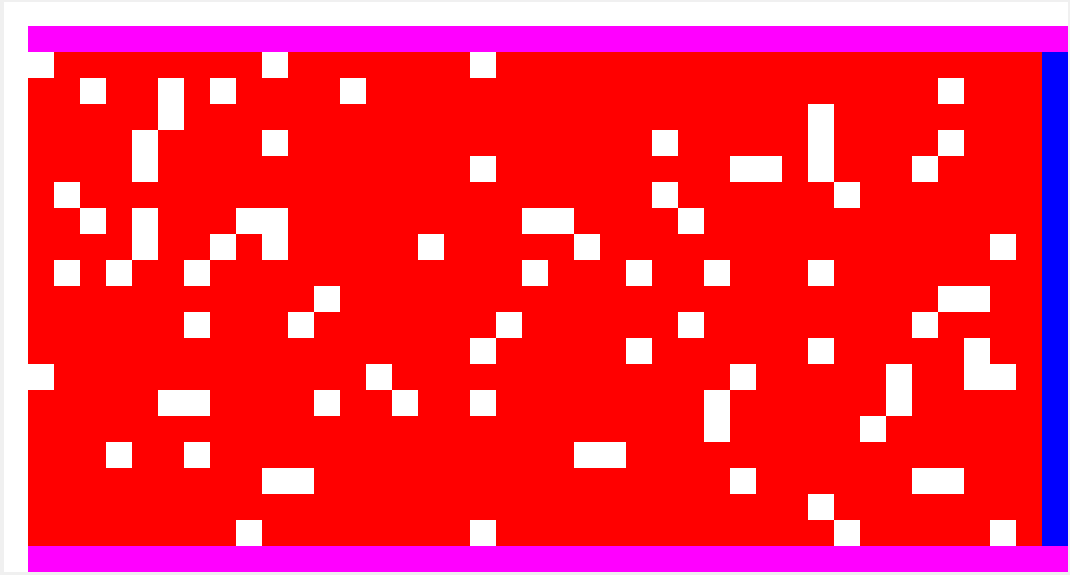
\includegraphics[width=\textwidth]{pictures/test2_6.png}
    \caption{$Density = 6 P/m^2$}
    \label{fig:test2_6}
  \end{subfigure}  
  \caption{Visualization of Test 2 in Task 5}
  \label{fig:test2}
\end{figure}

\begin{figure}[htbp]
      \centering
      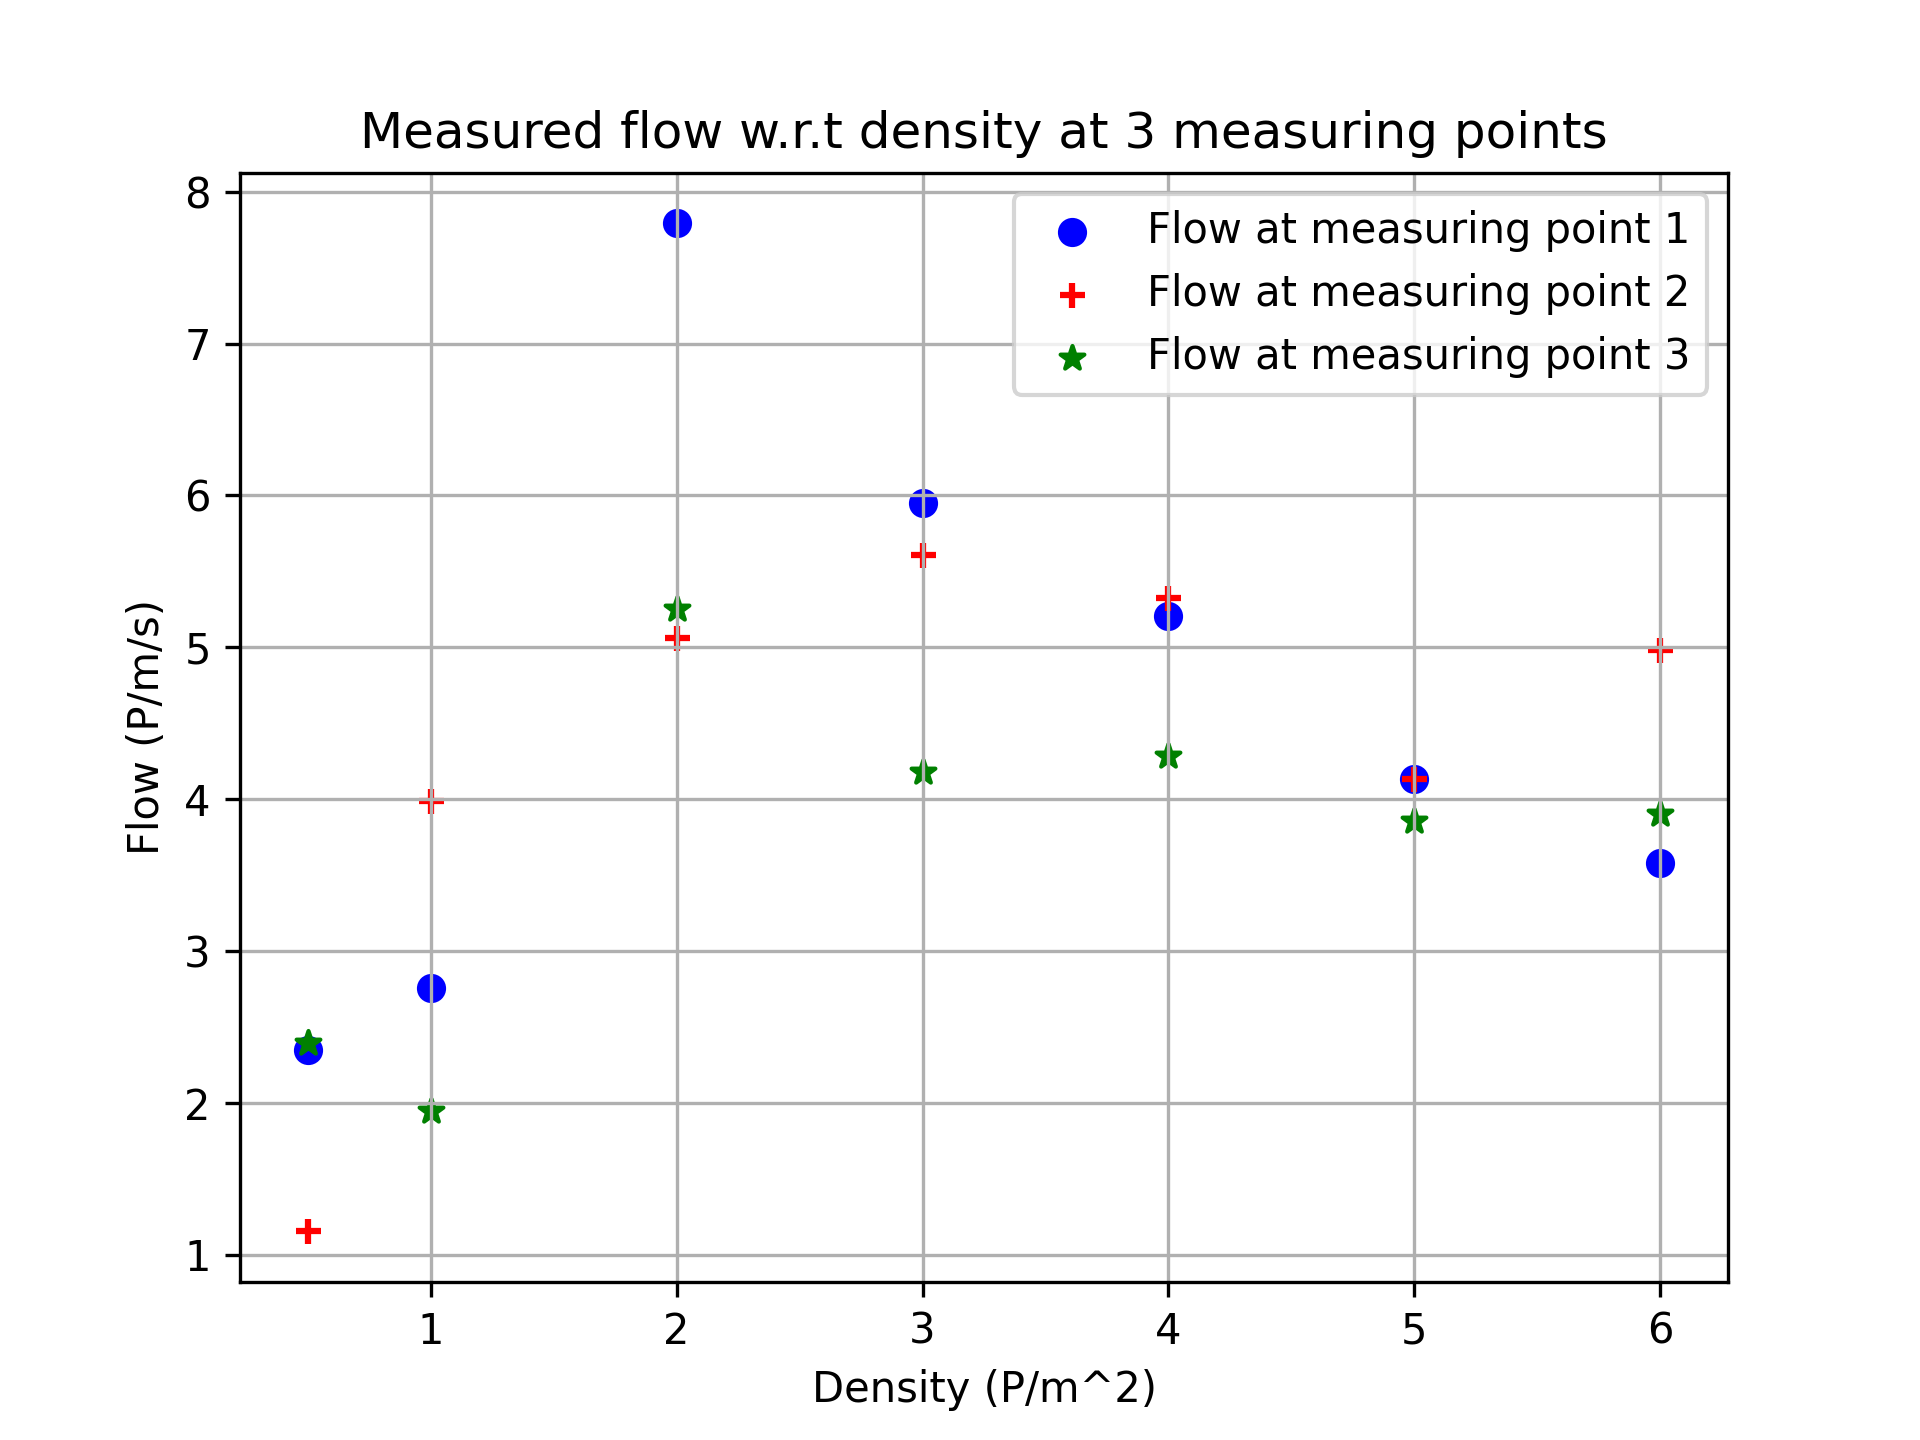
\includegraphics[width=0.9\linewidth]{pictures/measured_flow_density.png}
      \caption{Measured flows w.r.t density at 3 measuring points}
      \label{fig:measured_flow_density}
\end{figure}

\subsection{Test 3: RiMEA Scenario 6}

\subsubsection{Setup of Scenario}

A group of twenty uniformly distributed pedestrians, heading toward a left-turning corner (as shown in \autoref{fig:test3_setup})\cite{RimeaGuidelines2016}, will navigate around it successfully without intersecting any walls. The cell size is still $0.4m \times 0.4m$. The scenario is made up of $40 \times 40$ cells and the pedestrians are uniformly placed at bottom left.

\begin{figure}
    \centering
    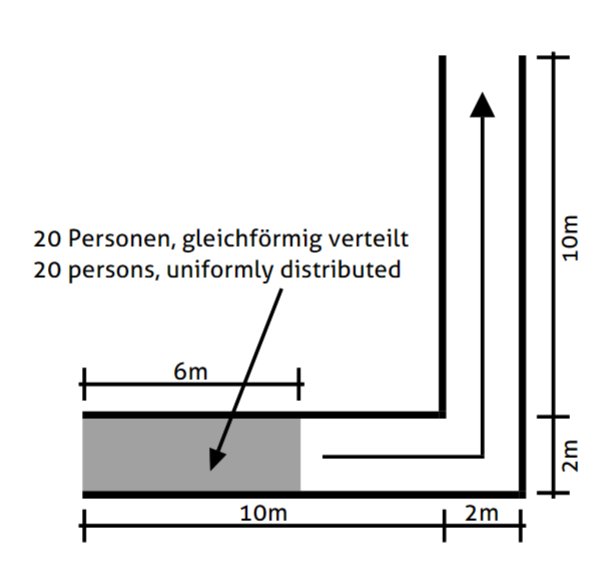
\includegraphics[width=0.5\linewidth]{pictures/test3_setup.png}
    \caption{The setup of Test 3 in Task 5}
    \label{fig:test3_setup}
\end{figure}

\subsubsection{Results of Simulation}

According to \autoref{fig:test3}, the crowd turns left successfully without getting through the walls and arrives at the targets as planned, which indicates that the algorithm passes Test 3.

\begin{figure}[htbp]
  \centering
  \begin{subfigure}[b]{0.31\textwidth}
    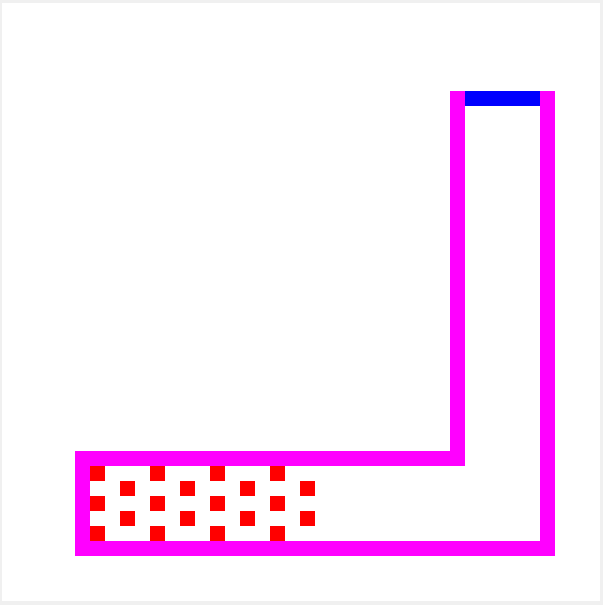
\includegraphics[width=\textwidth]{pictures/test3_initial.png}
    \caption{Initial state}
    \label{fig:test3_initial}
  \end{subfigure}
  \begin{subfigure}[b]{0.31\textwidth}
    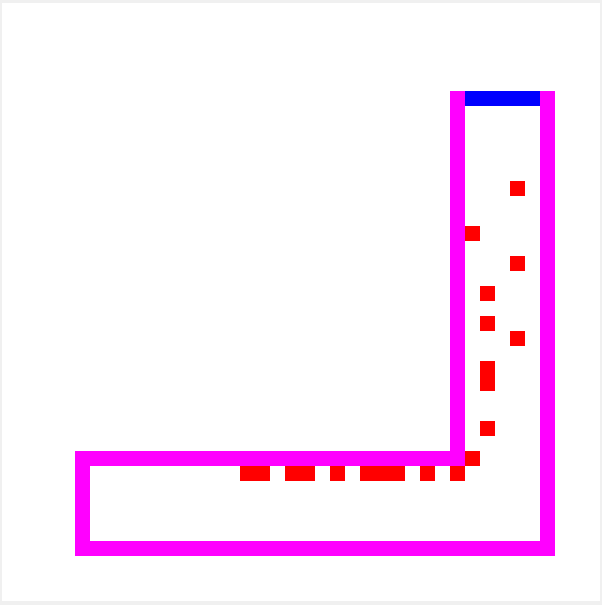
\includegraphics[width=\textwidth]{pictures/test3_intermediate.png}
    \caption{Intermediate state}
    \label{fig:test3_intermediate}
  \end{subfigure}
  \begin{subfigure}[b]{0.31\textwidth}
    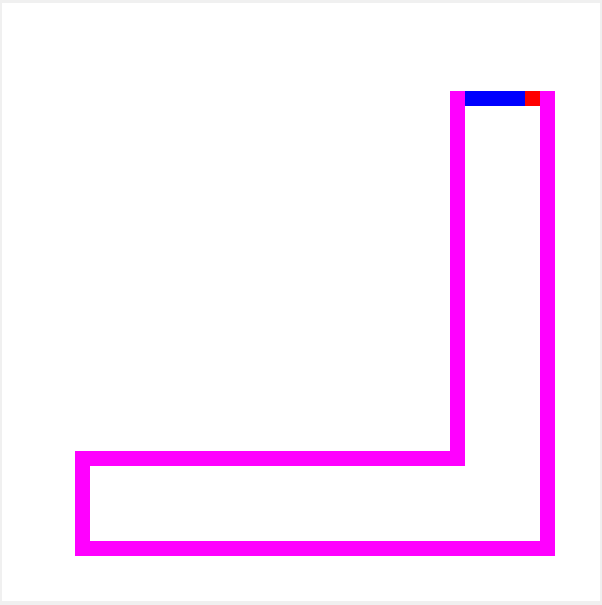
\includegraphics[width=\textwidth]{pictures/test3_end.png}
    \caption{Final state}
    \label{fig:test3_end}
  \end{subfigure}
  \caption{Visualization of Test 3 in Task 5}
  \label{fig:test3}
\end{figure}

\subsection{Test 4: RiMEA Scenario 7}

\subsubsection{Setup of Scenario}

In Test 4, 50 pedestrians are facing 50 targets $20m$ away from them. The cell size is $1m \times 1m$ for simplification. The pedestrians are randomly sampled from configs/rimea\_7\_speeds.csv, where each pedestrian is preassigned a speed correlated to the age, as shown in \autoref{fig:speed_age}\cite{weidmann1993transporttechnik}. The pedestrians are supposed to walk straight towards targets so the speed is computed via walking distance ($50m$) divided by time spent by each pedestrian. It is required to demonstrate that the distribution of walking speeds observed in the simulation aligns with the distribution presented in \autoref{fig:speed_age}.

\begin{figure}
    \centering
    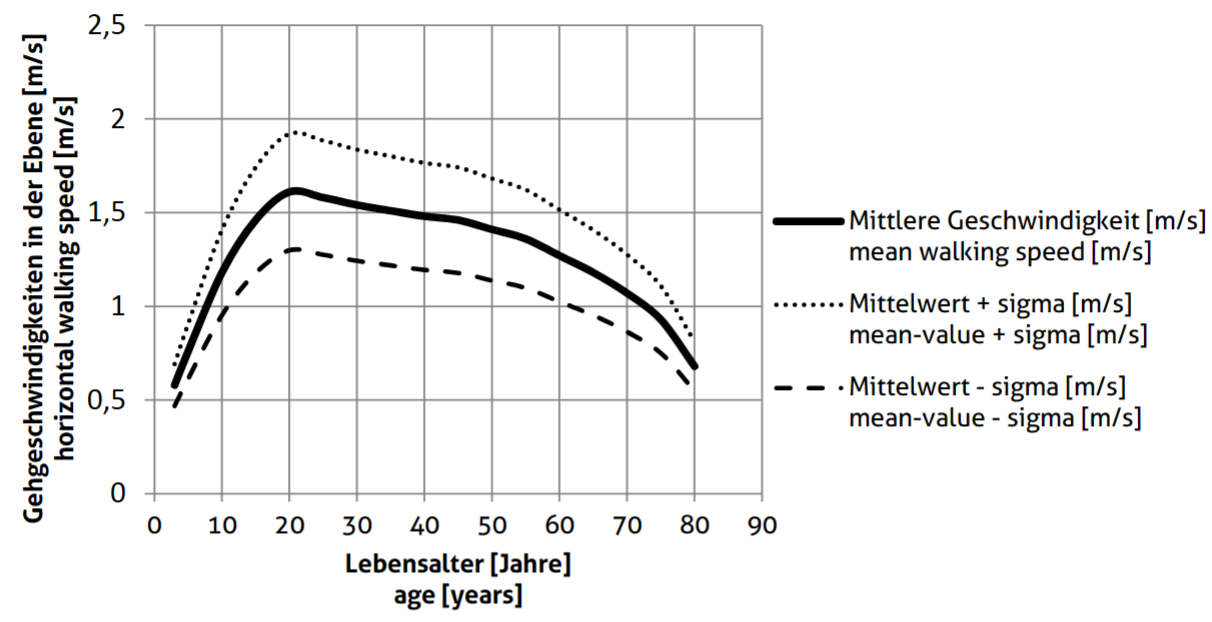
\includegraphics[width=0.75\linewidth]{pictures/speed_age.png}
    \caption{Walking speed in the plane as a function of age based on Weidmann}
    \label{fig:speed_age}
\end{figure}

\subsubsection{Results of Simulation}

\autoref{fig:measured_speed_age} compares the distribution of measured speeds in Test 4 and preassigned speeds from rimea\_7\_speeds.csv. It shows that most of the measured speeds are below the preassigned speeds. However, the preassigned speeds will be approximately aligned with the measured ones if given an offset of $-0.33 m/s$. The potential reason is that the pedestrians are placed in a line in the beginning, which makes them have an effect on each other at the start. They tend to avoid colliding with each other, which causes a delay of a few seconds. After the crowd scatters, the influence of avoidance becomes very weak and the pedestrians can move with preassigned speeds respectively. Therefore, an offset exists together with outliers, while the distribution in practice is roughly consistent with the ideal distribution.

\begin{figure}
    \centering
    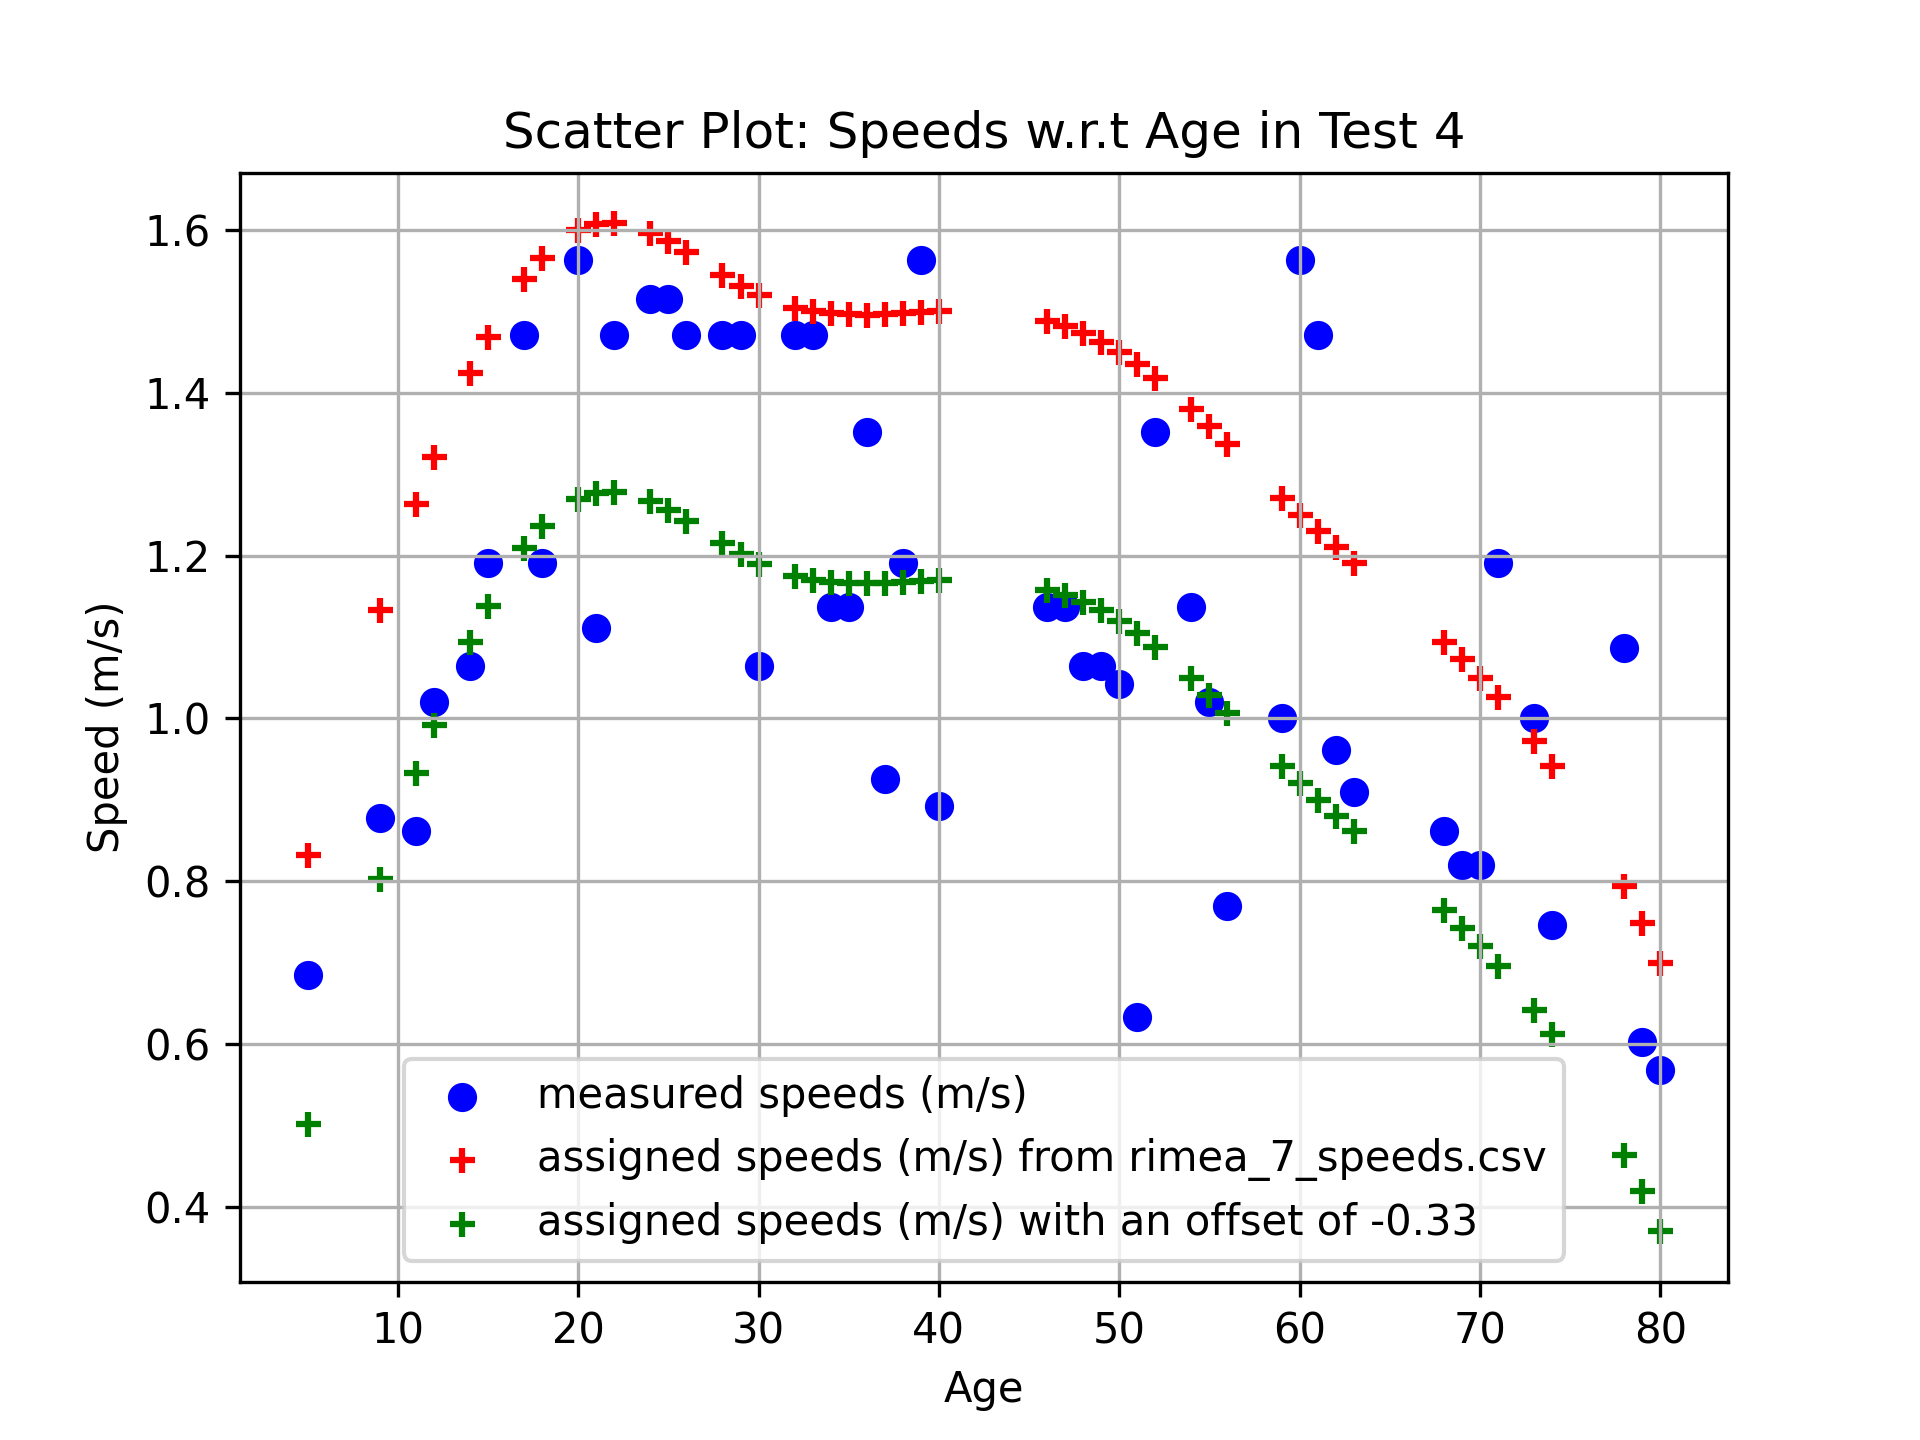
\includegraphics[width=1\linewidth]{pictures/measured_speed_age.png}
    \caption{Distribution of measured speeds in Test 4 and preassigned speeds from rimea\_7\_speeds.csv w.r.t age}
    \label{fig:measured_speed_age}
\end{figure}

\end{task}

\bibliographystyle{plain}
\bibliography{ref}

\end{document}